% !TeX spellcheck = de_DE
\section{Marketing}
\subsection{Entwicklung}
\subsubsection{Bis 1970er}
\begin{itemize}
	\item Nachfrageüberhang auf vielen Märkten
	\item Fokus auf Optimierung der Ausschöpfung von Produktionskapazitäten.
	\item Marktseitige Aktivitäten = effiziente Leistungsdistribution an Kunden
\end{itemize}
\textbf{--- KEIN MARKETING NOTWENDIG}

\subsubsection{Ab 1970er}
\begin{itemize}
	\item Nachfrageüberhang verschwunden - Marktsättigung (steigender Wettbewerb, Internationalisierung, abnehmende Innovationsgrade
	\item Wandelnde Märkte
	\item «Käufermärkte» (bessere Position auf Seite der Käufer)
	\item Notwendigkeit, Kundenwünsche bereits innerhalb des Entwicklungs- und Produktionsprozesses zu berücksichtigen
\end{itemize}
\textbf{--- MARKETING NOTWENDIG}

\subsubsection{Entwicklung einer neuen Unternehmensaufgabe}
\begin{itemize}
	\item Eigene unternehmerische Funktion
	\item Ziel: Ausrichtung aller unternehmerischen Aktivitäten an den Markterfordernissen (Beschaffungsmarketing allerdings selten)
	\item Weit mehr als nur die Erweiterung des Vertriebs bzw. der traditionellen Vertriebsabteilungen
	\item Zunächst Verbreitung im B2C-Bereich bei physischen Produkten. Erst später auch im B2B-Bereich und bei Dienstleistungen.
\end{itemize}

\subsection{Definition}
Marketing ist die Ausrichtung aller unternehmerischen Aktivitäten an den Markterfordernissen. \\
Marketing ist die
\begin{itemize}
	\item Planung, Organisation, Implementierung und Kontrolle (Managementaspekt)
	\item aller Aktivitäten mit der Absicht der Erreichung qualitativer und/oder quantitativer Vorgaben (Entscheidungsaspekt)
	\item durch Auswahl und Aufbau, Unterhalt und Referenzierung, Ausbau und Intensivierung bzw. Wiederherstellung oder Ausgrenzung von Geschäftsbeziehungen (Pflegeaspekt)
	\item mit jeweils relevanten Zielgruppen in Absatz, Beschaffung, Produktion, Umfeld und Medien (Anspruchsgruppenaspekt).
\end{itemize}

\subsection{Zielsetzung / Wettbewerbsvorteile}
\textbf{Grundsätzliche Zielsetzung:} Ausrichtung aller unternehmerischen Aktivitäten an den Markterfordernissen. \\
\textbf{Umsetzung:} Komparative Wettbewerbsvorteile, «Besser sein» im Vergleich zum Wettbewerb \\
Wettbewerbsvorteile:
\begin{enumerate}
	\item Müssen bedeutsam sein (insbesondere für Kaufentscheidung)
	\item Müssen wahrgenommen werden
	\item Müssen verteidigbar sein (z.B. Patente, Markenschutz, ...)
	\item Müssen effizient sein (Massnahmen dürfen nicht mehr kosten als sie nachher einbringen)
\end{enumerate}

\subsection{Elemente einer Marketing-Konzeption}
Realisierung von Wettbewerbsvorteilen durch bessere Ausrichtung der unternehmerischen Aktivitäten auf Marktanforderungen erfolgt in einem ineinandergreifenden Prozess von verschiedenen Elementen:\\
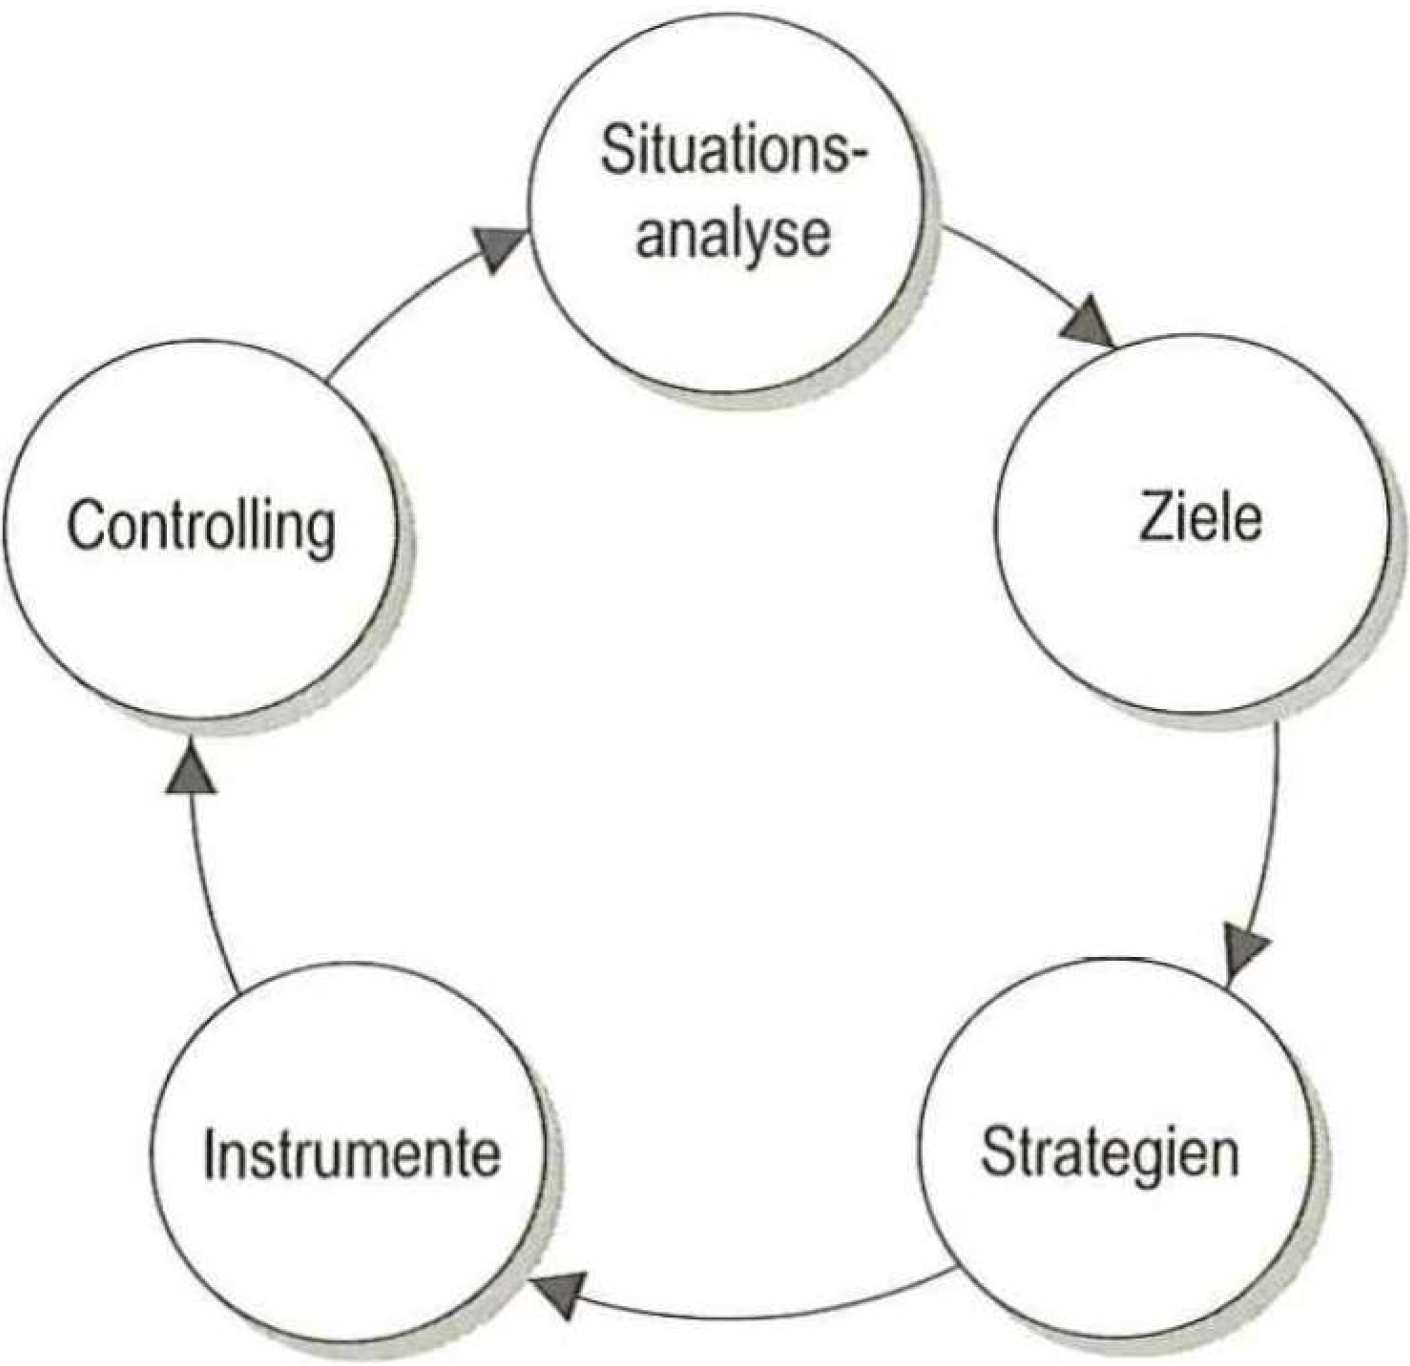
\includegraphics[width=0.2\linewidth]{images/elemente_marketing}

\subsection{Situationsanalyse}
\subsubsection{Aufgabe}
\begin{itemize}
	\item Zielgerichtete Beschaffung, Strukturierung und Auswertung aller für die anschliessende Ableitung von Marketingentscheidungen benötigten Informationen.
	\item Definition von IST und SOLL Positionierungen der eigenen Angebote
	\item Ausgangspunkt für weitere Erarbeitung von Zielen, Strategien und Instrumenten
\end{itemize}

\subsubsection{Analyseperspektiven}
\begin{multicols}{3}
	\begin{enumerate}
		\item Nachfrager
		\item Wettbewerb
		\item Ressourcen
	\end{enumerate}
\end{multicols}
Ziel: eigene Positionierung

\subsubsection{Nachfrageranalyse}
\textbf{Aufgabe}
\begin{itemize}
	\item Beschaffung und Interpretation aller im Zusammenhang mit dem Kaufverhalten von aktuellen und potenziellen Nachfragern stehenden Informationen.
\end{itemize}

\textbf{Unterscheidung nach}
\begin{enumerate}
	\item Individuelles Kaufverhalten
	\begin{itemize}
		\item persönliches Kaufverhalten (B2C)
		\item organisationales Kaufverhalten (B2B)
	\end{itemize}
	\item Aggregiertes Kaufverhalten (Marktsegmente)
\end{enumerate}

\paragraph{SOR}
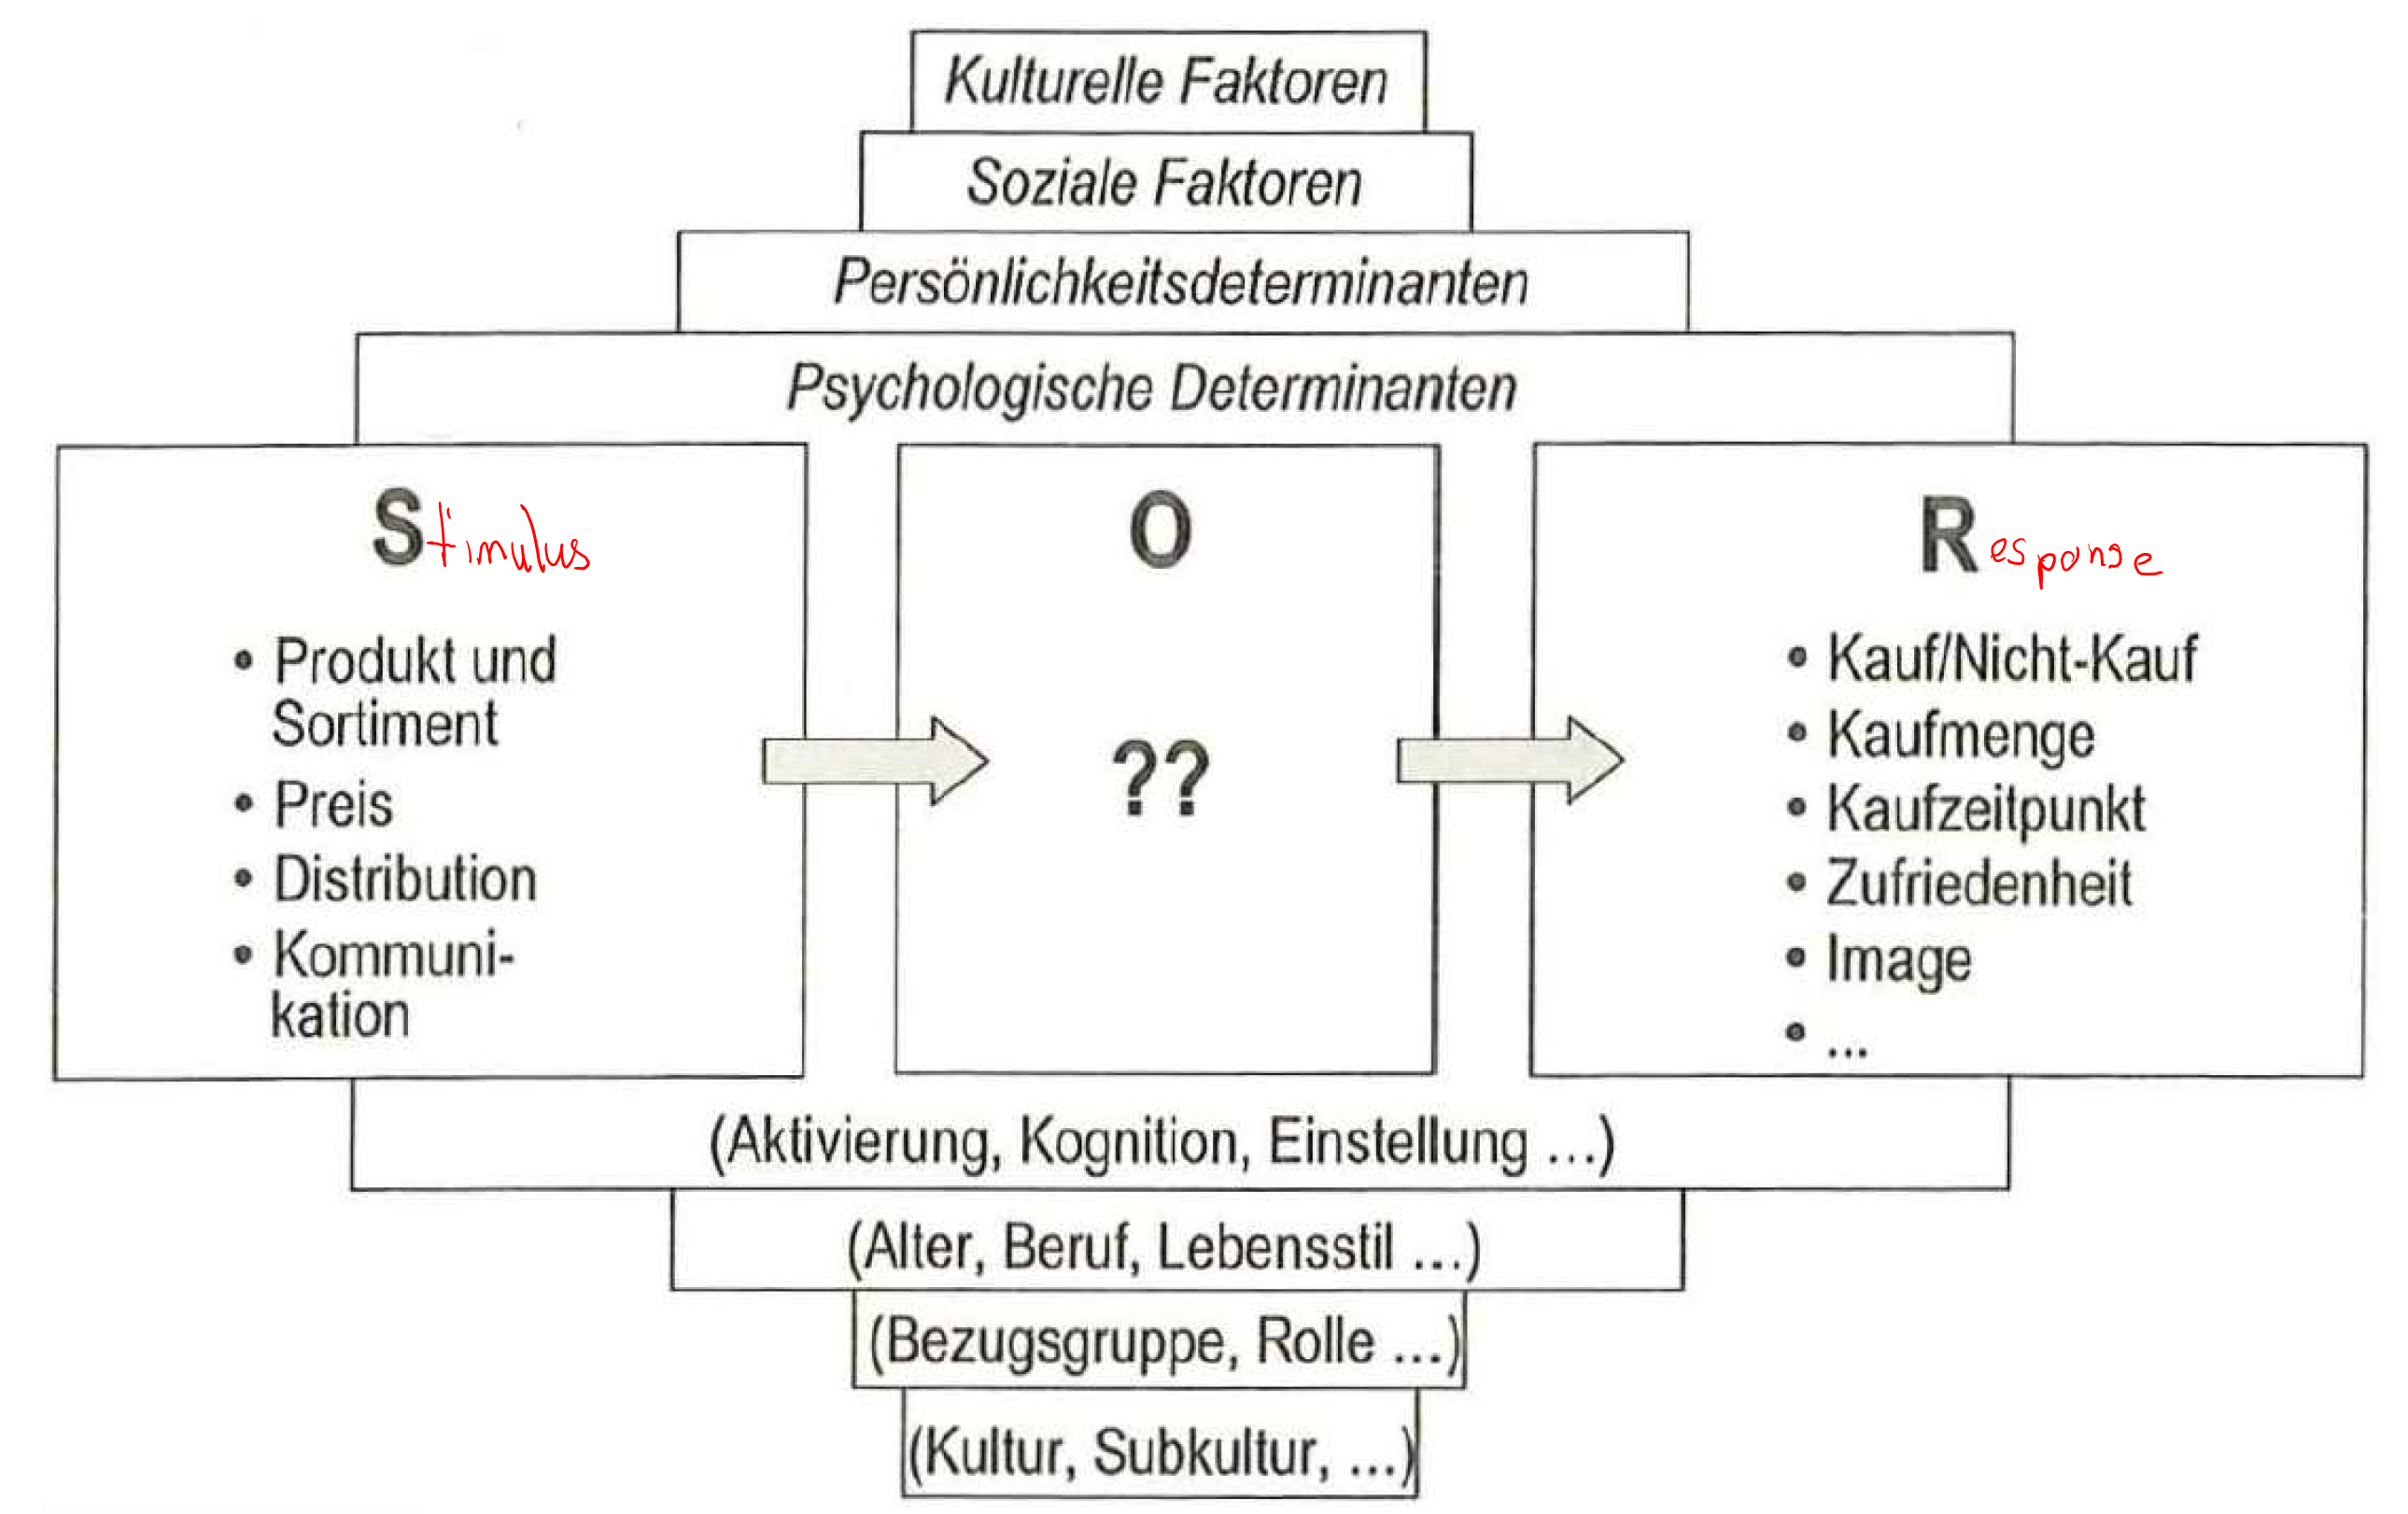
\includegraphics[width=0.4\linewidth]{images/sor}

\paragraph{Buying Center}
«Buying Center» als Perspektive der Analyse organisationalen Kaufverhaltens.
\begin{itemize}
	\item Industriegüter / B2B
	\begin{itemize}
		\item Einzelne, organisationale Nachfrager im Mittelpunkt der Analyse
		\item Leistungen / Gegenleistungen werden bilateral ausgehandelt
		\item Neben allgemeiner Marktbearbeitung besondere Bedeutung von Vertriebsmitarbeitern / -einheiten
		\item Komplexe Entscheidungswege mit mehreren Beteiligten (auf unterschiedlichen Hierarchieebenen) auf Nachfragerseite
	\end{itemize}
	\item Vorgehen
	\begin{itemize}
		\item Ziel: Systematische Bearbeitung des Nachfragers
		\item Identifikation und Strukturierung des Einkaufsgremiums (Buying Centers) nach Aufgaben und Rollen
		\item Systematische Erfassung und zentrale Speicherung im Vertrieb (white books)
	\end{itemize}
	\item «Buying Center» sind Organisationseinheiten
	\begin{itemize}
		\item die aus Individuen und Teileinheiten der Organisation des	Nachfragers zusammengesetzt sind und die Kaufprozesse durchführen
		\item Mögliche Rollen der Mitglieder sind:
		\begin{enumerate}
			\item Nutzer
			\item Beeinflusser (z.B. Techniker erstellen Spezifikationen)
			\item Einkäufer (z.B. Berechtigung zur Lieferantenauswahl)
			\item Entscheider (z.B. Einkaufsabteilungen)
			\item Informationsselektierer (z.B. Beteiligte an Informationswegen)
		\end{enumerate}
	\end{itemize}
\end{itemize}

\paragraph{aggregierten Nachfrageanalyse}
\begin{itemize}
	\item Ähnlichkeit des Kaufverhaltens verschiedener Nachfrager
	\item Abgrenzung in sich homogener Teilmärkte (Segmente)
\end{itemize}

\paragraph{Marktsegmente}
\begin{itemize}
	\item Ausrichtung an nachfrageseitigen Merkmalen mit Einfluss auf /	Zusammenhang mit:
	\begin{itemize}
		\item Kaufverhalten
		\item Nutzungsverhalten
		\item Organisationales Beschaffungsverhalten
	\end{itemize}
\end{itemize}

\subsubsection{Wettbewerbsanalyse}
\begin{itemize}
	\item Abgrenzung des Wettbewerbs
	\begin{itemize}
		\item Voraussetzung: Identifikation des relevanten Marktes
		\item Gleichbedeutend mit: Wettbewerbern, die von Kunden als in Frage kommende Konkurrenten wahrgenommen werden
	\end{itemize}
	\item  Sachliche Abgrenzung
	\begin{itemize}
		\item Inwieweit nehmen Kunden generell andere Leistungen von Wettbewerbern als relevante Substitutionsmöglichkeiten wahr?
	\end{itemize}
	\item  Zeitliche Abgrenzung
	\begin{itemize}
		\item Zwischen welchen zu verschiedenen Zeitpunkten getroffenen Kaufentscheidungen von Kunden bestehen Substitutionsmöglichkeiten? (z.B. Kunden warten bis das neue iPhone vorgestellt wurde bevor sie ein neues handy kaufen.)
	\end{itemize}
	\item  Räumliche Abgrenzung
	\begin{itemize}
		\item Inwieweit nehmen Kunden Wettbewerber aus anderen Regionen / Ländermärkten als relevante Substitutionsmöglichkeiten wahr?
		\item Transport: Aufwand, Zeit, Kosten
	\end{itemize}
\end{itemize}

\paragraph{Branchenanalyse}
\begin{itemize}
	\item Identifikation von Treibern/Einflüssen, die für alle Wettbewerber in einer Branche gelten
	\item Z.B. Branchenstrukturanalyse (Five Forces) nach Porter
\end{itemize}

\paragraph{Segmentanalyse (Strategische Gruppen Analyse)}
\begin{itemize}
	\item Analyse einzelner Marktsegmente (Strategische Gruppen)
	\item Identifikation von Clustern von Konkurrenten, die sich in ähnlichen strategischen Ausgangsituation befinden.
	\item Entsprechend ist auch ein ähnliches Wettbewerbsverhalten zu erwarten
\end{itemize}

\paragraph{Konkurrenzanalyse}
\begin{itemize}
	\item Form der Wettbewerbsanalyse, die am weitesten geht
	\item Umfassende Analyse besonders relevanter Konkurrenten
	\item Besondere Herausforderung: Beschaffung relevanter Informationen
	\item Systematische Erfassung intern und extern verfügbarer Informationen über relevante Konkurrenten
	\item Nutzung zur Abschätzung deren zukünftigen Verhaltens
\end{itemize}
Ist je nachdem am Rand der Wirtschaftsspionage.

\subsubsection{Ressourcenanalyse}
\begin{itemize}
	\item Ziel
	\begin{itemize}
		\item Möglichst objektive Analyse der marktbezogenen Stärken und Schwächen des eigenen Unternehmens
	\end{itemize}
	\item Relative Untersuchung
	\begin{itemize}
		\item Beurteilung der eigenen Möglichkeiten im Vergleich zu den in der Wettbewerbsanalyse als relevant eingestuften Konkurrenten
		\item Benchmarking als geeignetes Analysetool
		\item Systematischer Vergleich zwischen Unternehmen(-seinheiten) anhand von standardisierten Vergleichsgrössen und Richtwerten
		\item Unterschiede werden gewichtet und zu einer Gesamteinschätzung der eigenen Ressourcen im Vergleich zum Wettbewerb aggregiert
	\end{itemize}
\end{itemize}

\subsubsection{Positionierung}
\begin{itemize}
	\item Ergebnisse der Nachfrager-, Wettbewerbs- und Ressourcenanalyse bilden Grundlage
	\item Positionierung des eigenen Unternehmens bzw. der angebotenen Leistungen
	\item Verortung in mehrdimensionalen Wahrnehmungs- / Präferenzräumen der Nachfrager: Darstellung meist zweidimensional als Grafik
\end{itemize}

\paragraph{Schritte}
\begin{enumerate}
	\item Auswahl der relevanten Perspektive(n) auf eigene Leistungen / Marken
	\item Auswahl relevanter Konkurrenz-Angebote
	\item Auswahl relevanter Dimensionen (Kaufverhalten)
	\item Bestimmung der Ausprägungen der eigenen Leistungen und die der Konkurrenz in Bezug auf die relevanten Dimensionen
\end{enumerate}

\paragraph{Ansätze}
\begin{multicols}{2}
	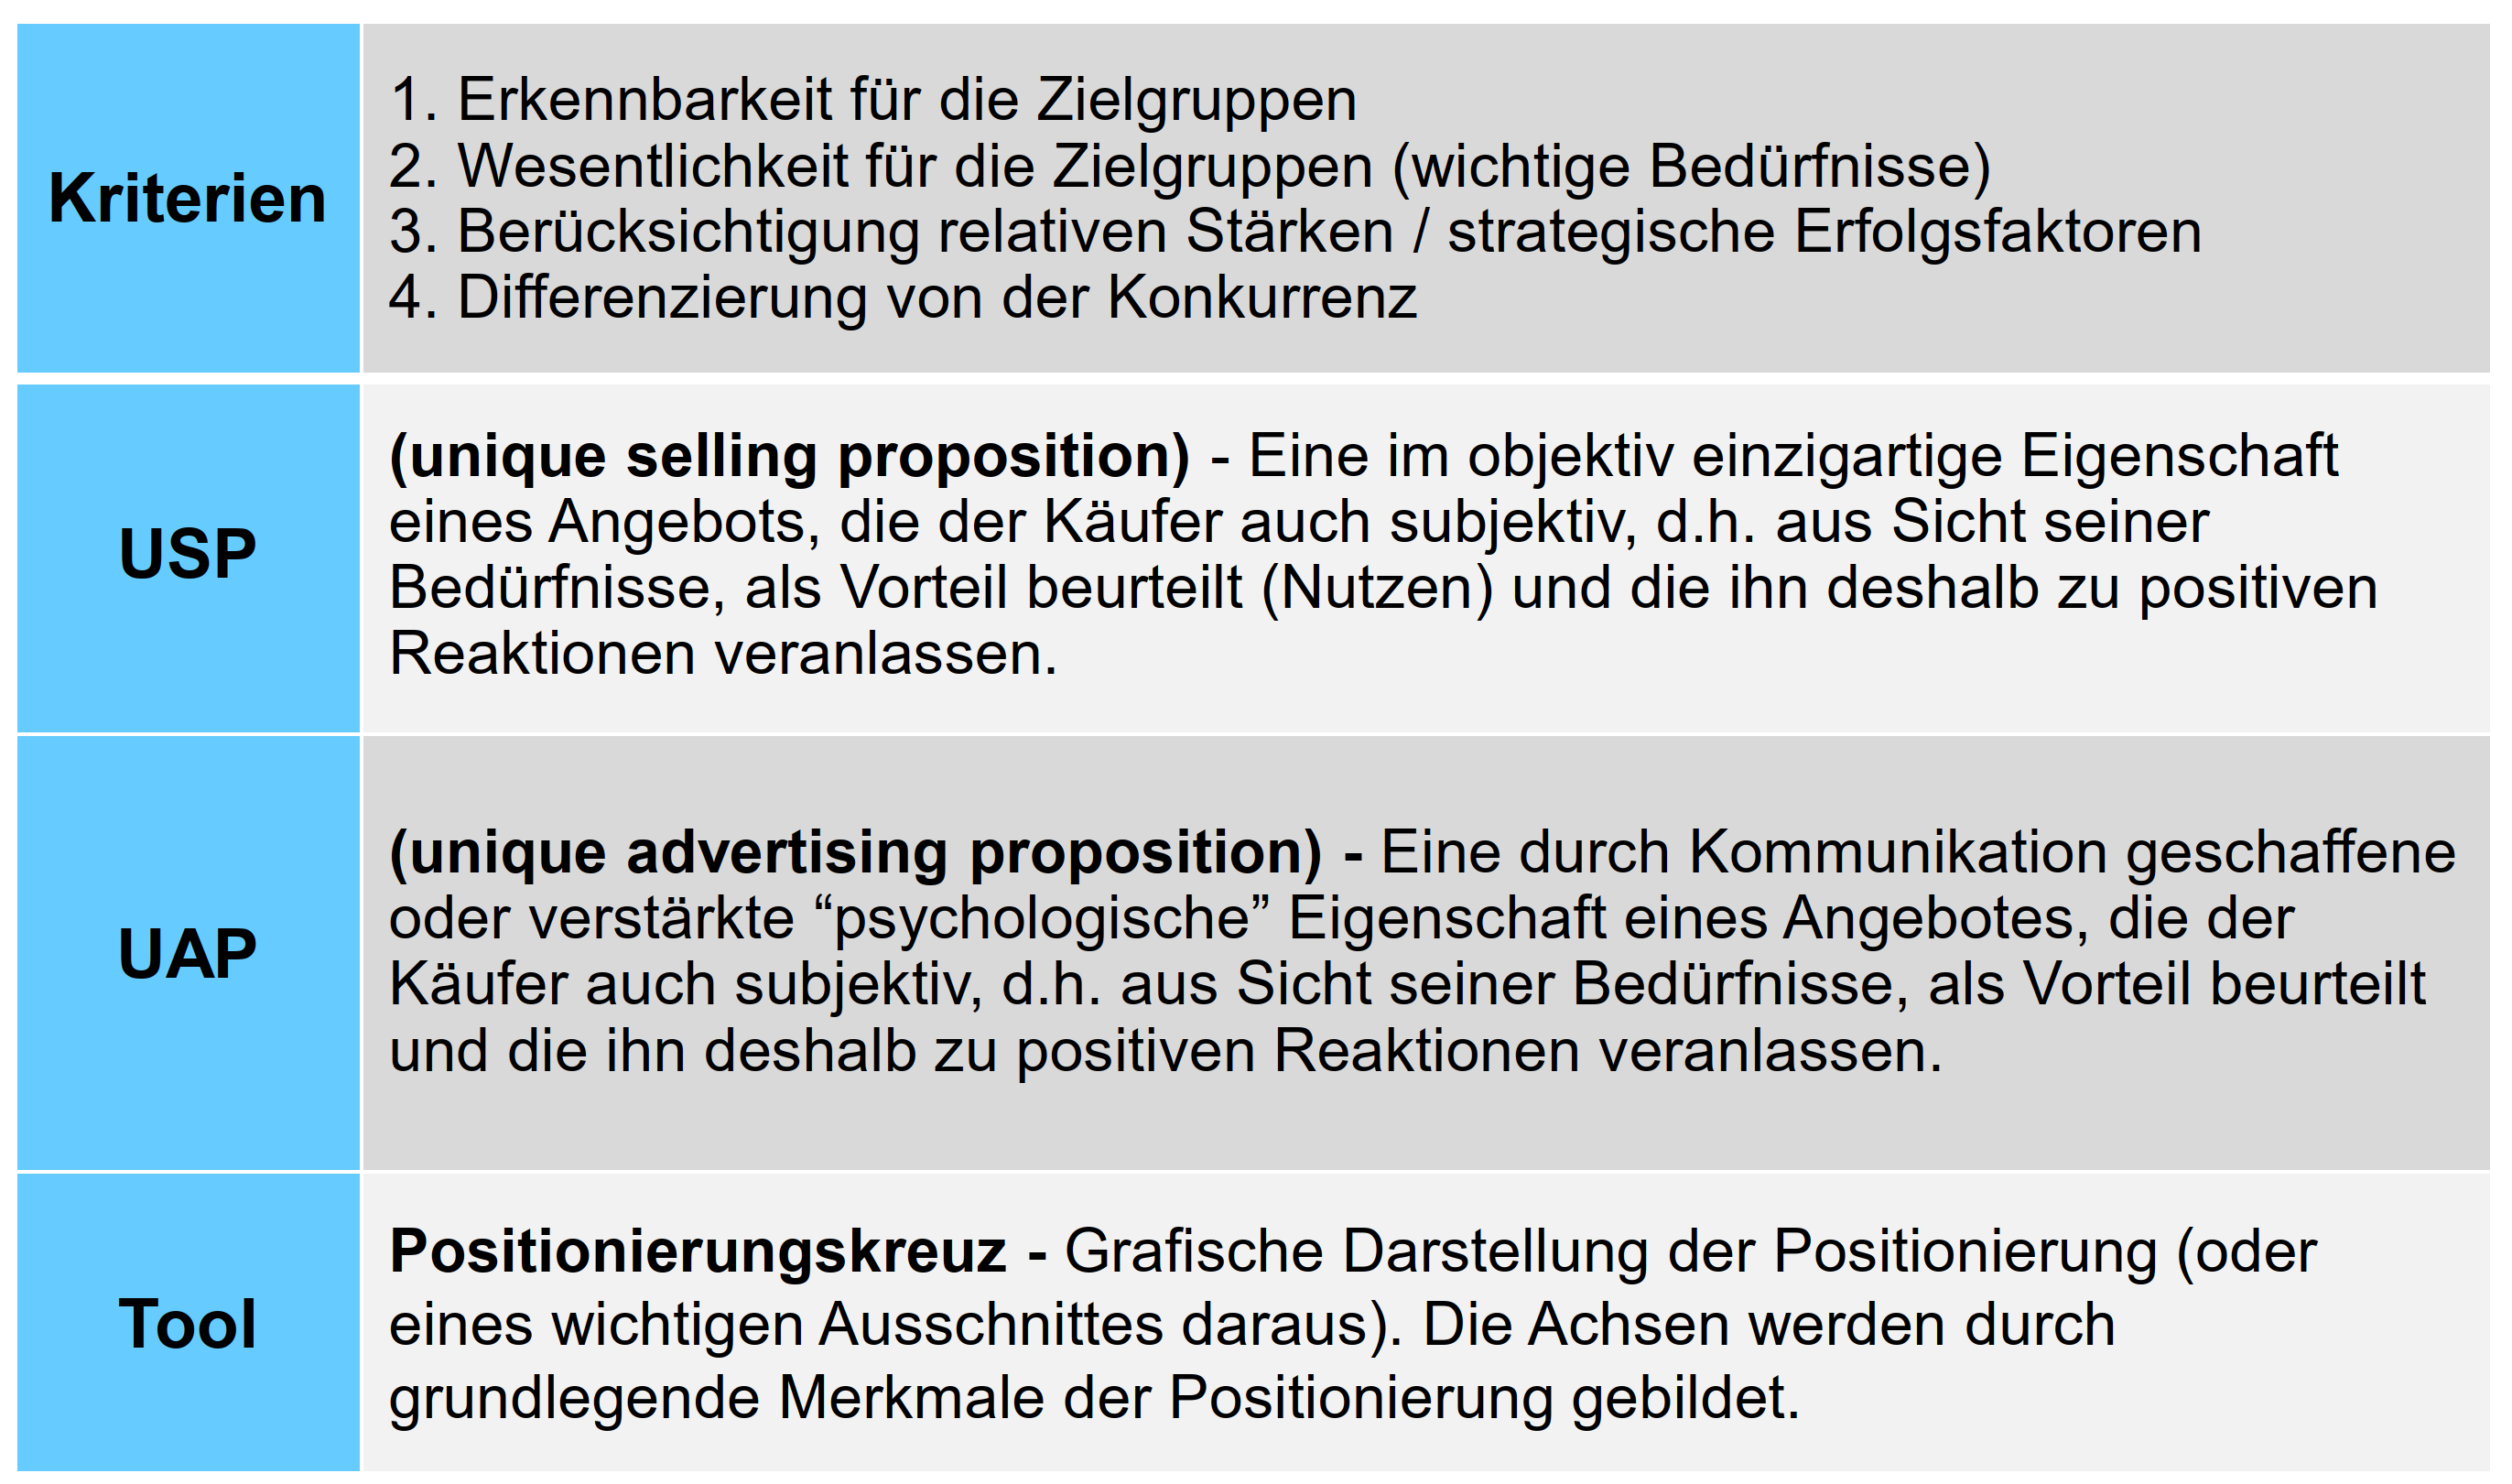
\includegraphics[width=1\linewidth]{images/ansatz_positionierung}
	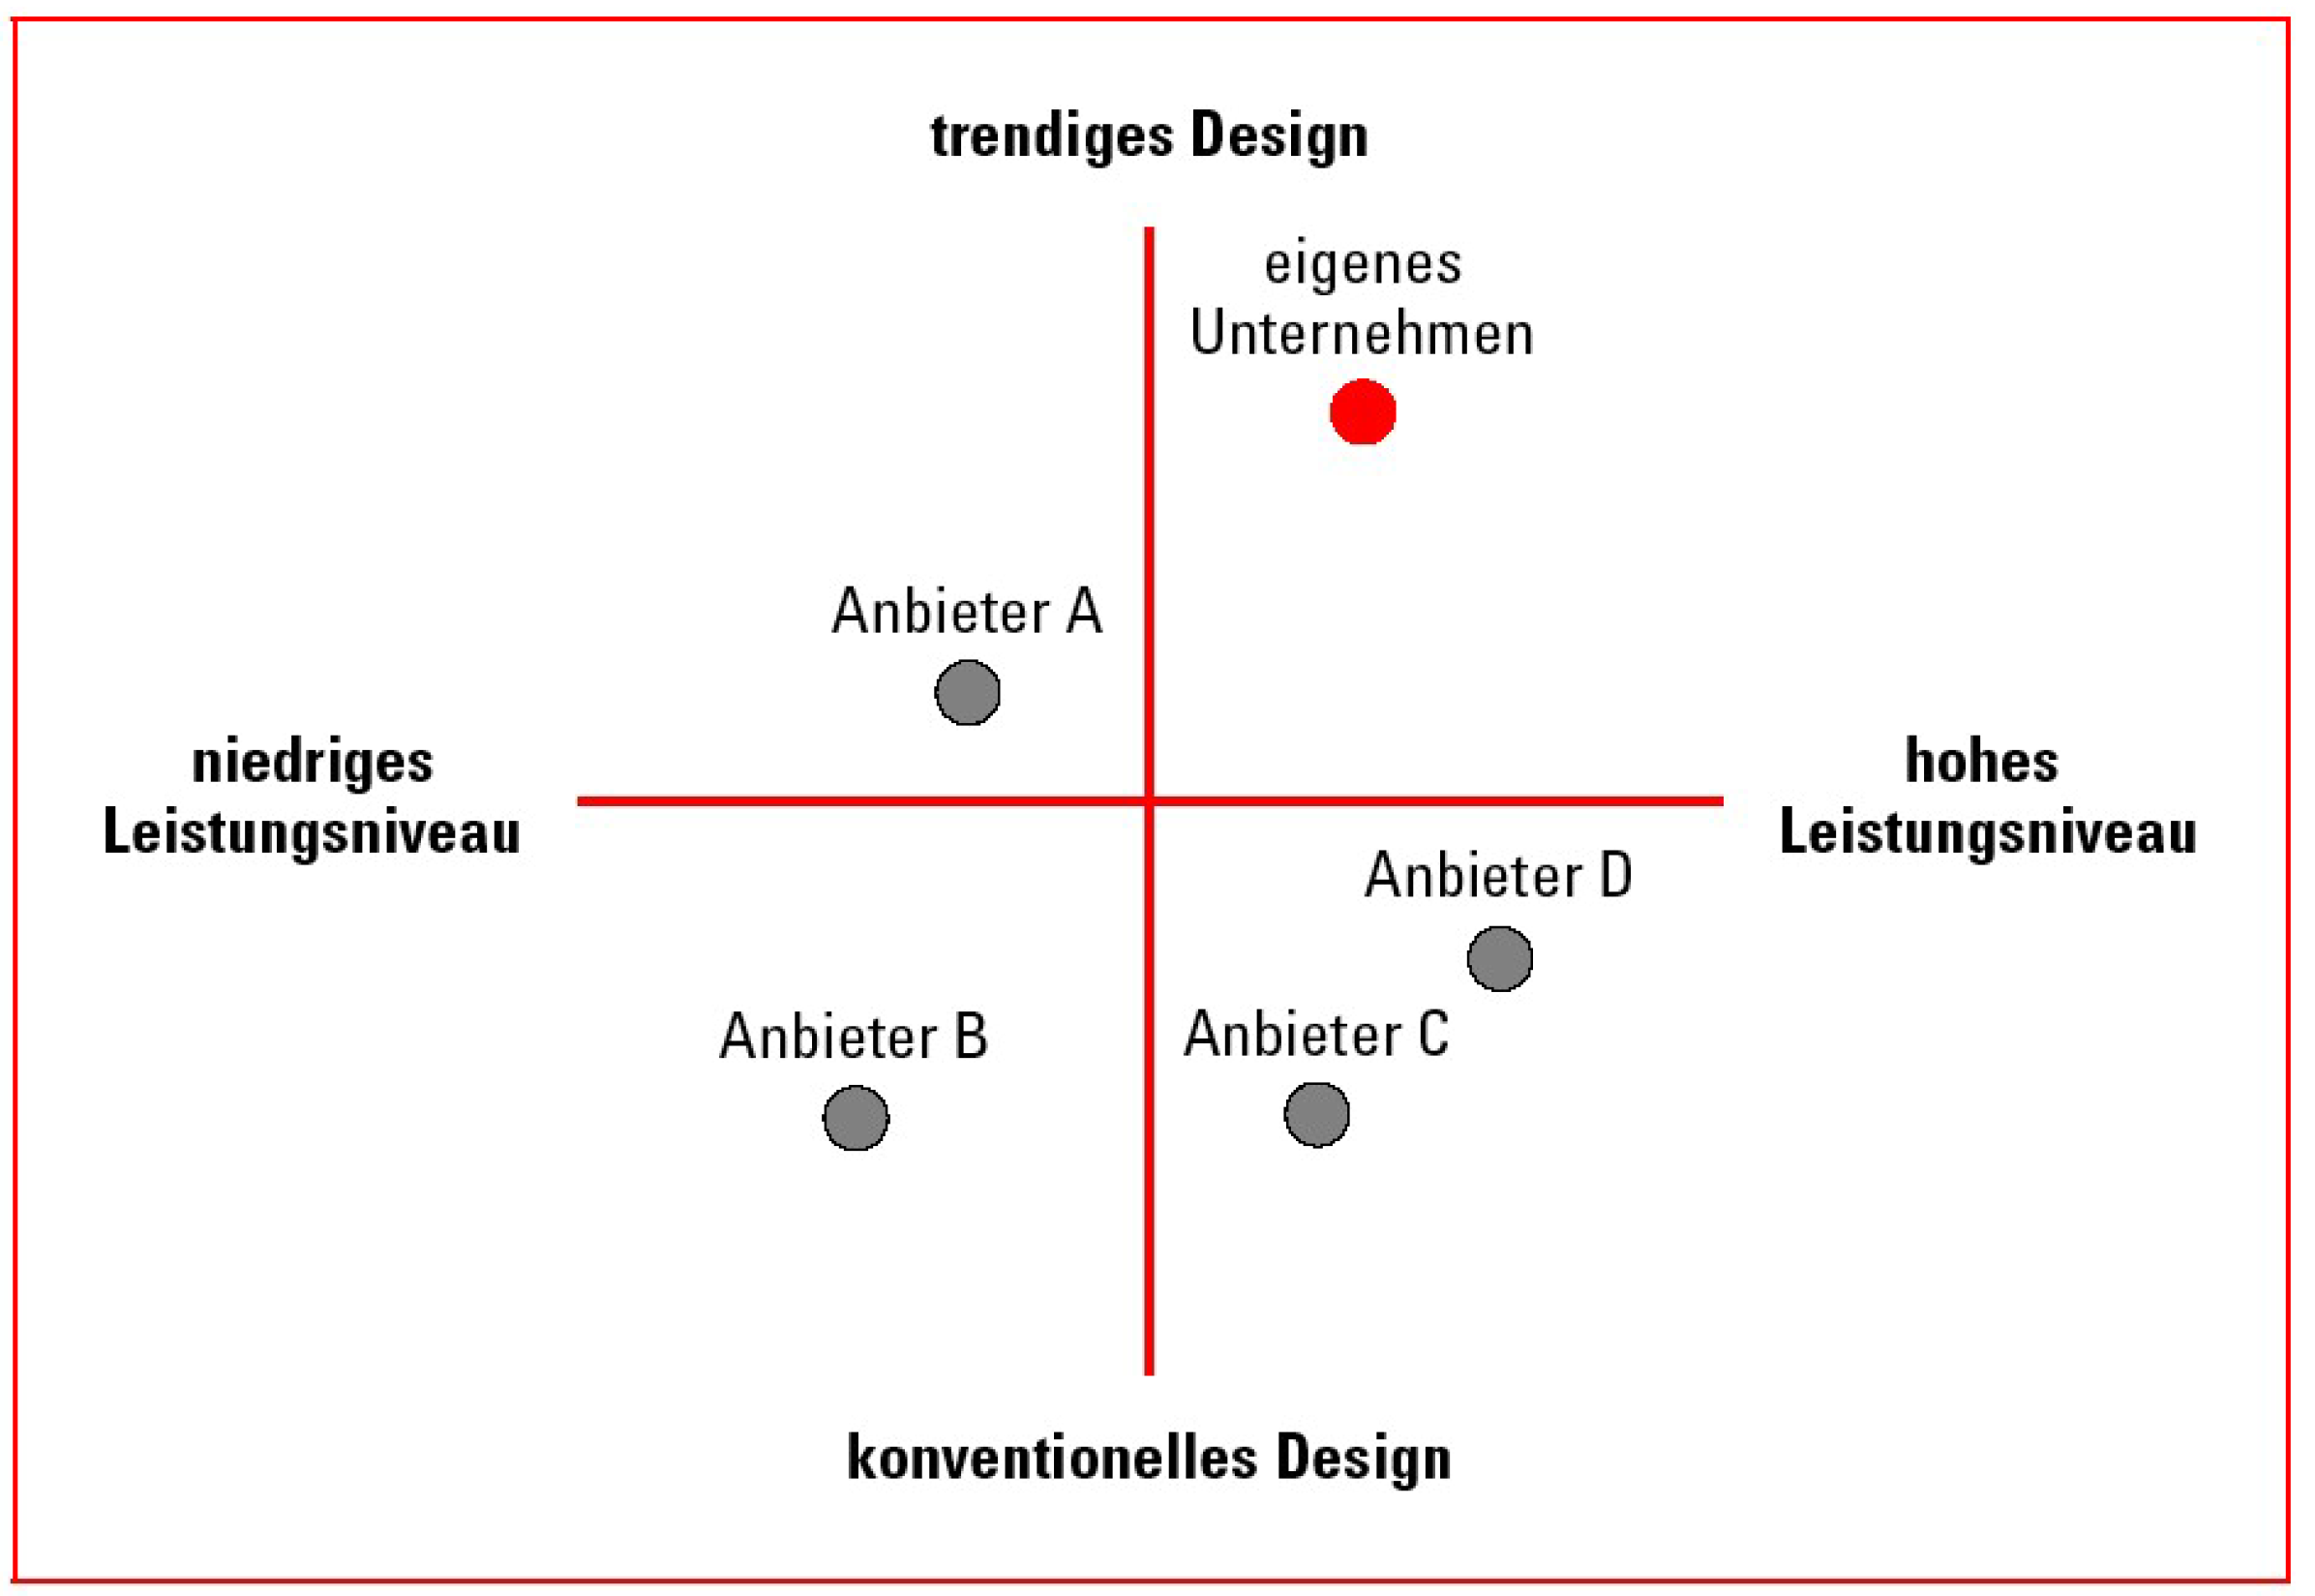
\includegraphics[width=0.9\linewidth]{images/positionierungskreuz}
\end{multicols}

\subsection{Marketing-Ziele}
\begin{itemize}
	\item Zweck
	\begin{itemize}
		\item Ziele sind Voraussetzung für effiziente und effektive Entwicklung von Strategien und Massnahmen
	\end{itemize}
	\item Zielformulierung
	\begin{itemize}
		\item Konkretisierung nach Inhalt, Ausmass, Zeit und Marktsegment.
		\item Inhalte müssen aus den Oberzielen des Unternehmens abgeleitet	werden.
		\item Lange Zeit wurden lediglich markterfolgsbezogene Ziele (Effektivität)	gesetzt: z.B.:
		\begin{itemize}
			\item Steigerung des relativen / absoluten Marktanteils
			\item Stabilisierung des am Markt erzielten Preisniveaus
		\end{itemize}
		\item Forderung nach maximaler Kundenorientierung
		\item Erst später Wandel zu stärkerer, ganzheitlichen Wertorientierung
	\end{itemize}
	\item Wertorientierung (Unternehmenswert nachhaltig steigern)
	\begin{itemize}
		\item Veränderung der Oberziele von Unternehmen auf stärkere, ganzheitliche Wertorientierung in den 1990er Jahren
		\item Alle Funktionen und Prozesse sind angehalten, den eigenen Wertbeitrag zum Unternehmen nachzuweisen: Auch das Marketing.
	\end{itemize}
	\item Effektivität / Effizienz
	\begin{itemize}
		\item Ziele zur Effektivität beim Unternehmensergebnis: Z.B.:
		\begin{itemize}
			\item Erzielte Deckungsbeiträge
			\item Umsatzrendite
		\end{itemize}
		\item Effizienzorientierte Ziele = Marketing-Kosten in Relation zu Effekten.
		\item Widersprüche zwischen (Effektivität und Effizienz von) Marketingmassnahmen z.B. Senkung des Produktpreises führt:
		\begin{enumerate}
			\item tendenziell zu höheren Absatzmengen
			\item ABER auch zu niedrigeren Margen
		\end{enumerate}
	\end{itemize}
\end{itemize}

\subsection{Marketing-Strategien}
\begin{itemize}
	\item Zweck
	\begin{itemize}
		\item Steuerung und Ausrichtung des Einsatzes der Marketing Instrumente im Hinblick auf die definierten Marketing Ziele.
		\item Längerfristige Gültigkeit - langfristige Ausrichtung der Marktaktivitäten an verbindlichem Handlungsrahmen.
	\end{itemize}
	\item Arten
	\begin{enumerate}
		\item Klassisch: Qualitätsführerschaft (Differenzierer) vs. Kostenführerschaft
		\item Zeitführerschaft
		\item Beziehungsmanagement / Relationship Management
		\begin{enumerate}
			\item Markenmanagement
			\item Kundenbindungsmanagement
		\end{enumerate}
	\end{enumerate}
\end{itemize}
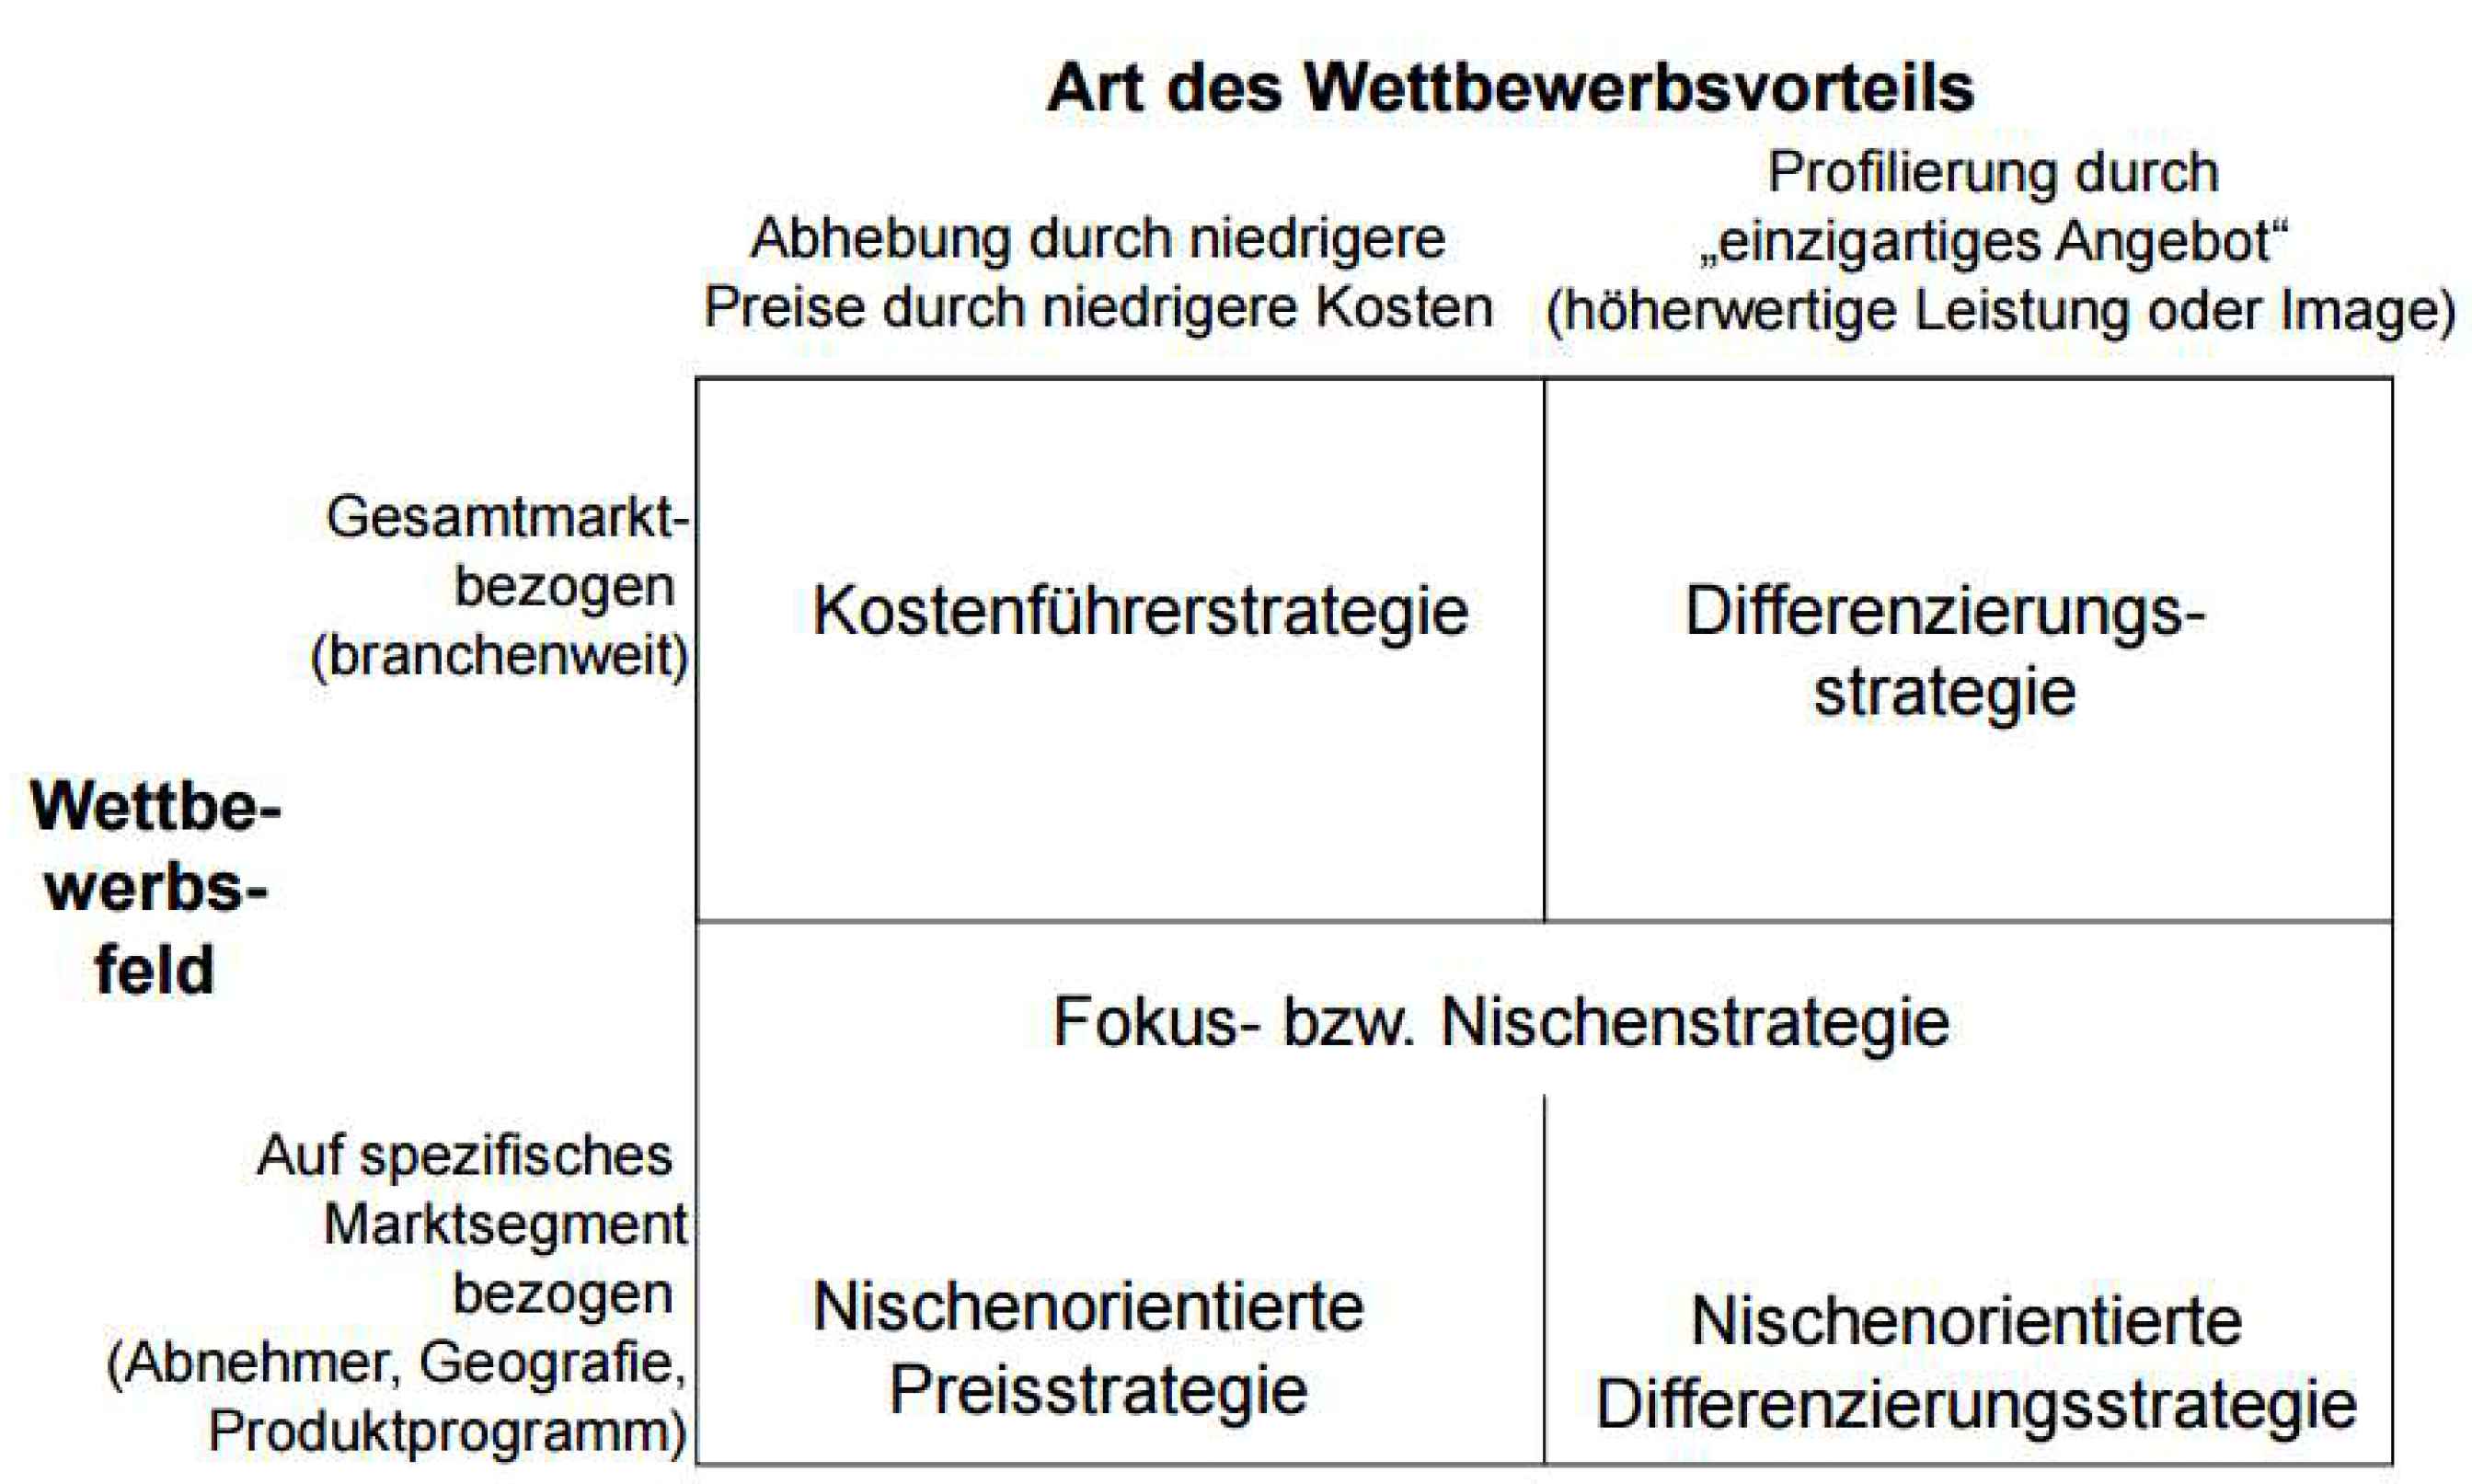
\includegraphics[width=0.5\linewidth]{images/marketing_klassisch}

\subsubsection{Zeitführerschaft}
\begin{itemize}
	\item Ziel
	\begin{itemize}
		\item Zum richtigen Zeitpunkt im Markt agieren
		\item Richtiger Zeitpunkt für Markteintritt / Marktaustritt
	\end{itemize}
	\item Markteintritt
	\begin{itemize}
		\item Besonders bedeutsam für junge, schnell wachsende Märkte
		\item Lebensdauer der Produkte reicht häufig nicht aus, um Entwicklungskosten zu amortisieren
		\item Um ein Jahr verzögerter Markteintritt kann Einbussen von bis zu 50\% des möglichen Produktvolumens zur Folge haben
	\end{itemize}
	\item Marktaustritt
	\begin{itemize}
		\item Eher bedeutsam für stagnierende Märkte und Produkte/Leistungen am Ende des Lebenszyklus
		\item Verzögerter Marktaustritt führt zu reduzierten Gewinnen bis hin zu Verlusten
	\end{itemize}
\end{itemize}

\subsubsection{Beziehungsmanagement}
\begin{itemize}
	\item Neue Perspektive
	\begin{itemize}
		\item Wechsel von sukzessiver Abfolge separater Einzeltransaktionen hin zu längerfristigen Beziehungen mit episodischen bzw. regelmässigen Transaktionen		
		\item Langfristige Bindung durch Bildung starker Marken und Steigerung der Kundenzufriedenheit
	\end{itemize}
	\item Funktionsweise
	\begin{itemize}
		\item Das Halten von bestehenden Kunden ist günstiger als das Gewinnen von neuen Kunden
		\item Akquisekosten (plus Haltekosten) können über mehrere Transaktionen amortisiert werden
		\item Ziel: Höhere Umsätze je Kunden (wiederholte Transaktionen, höhere Zahlungsbereitschaft, Cross Selling)
	\end{itemize}
\end{itemize}
\begin{multicols}{2}
	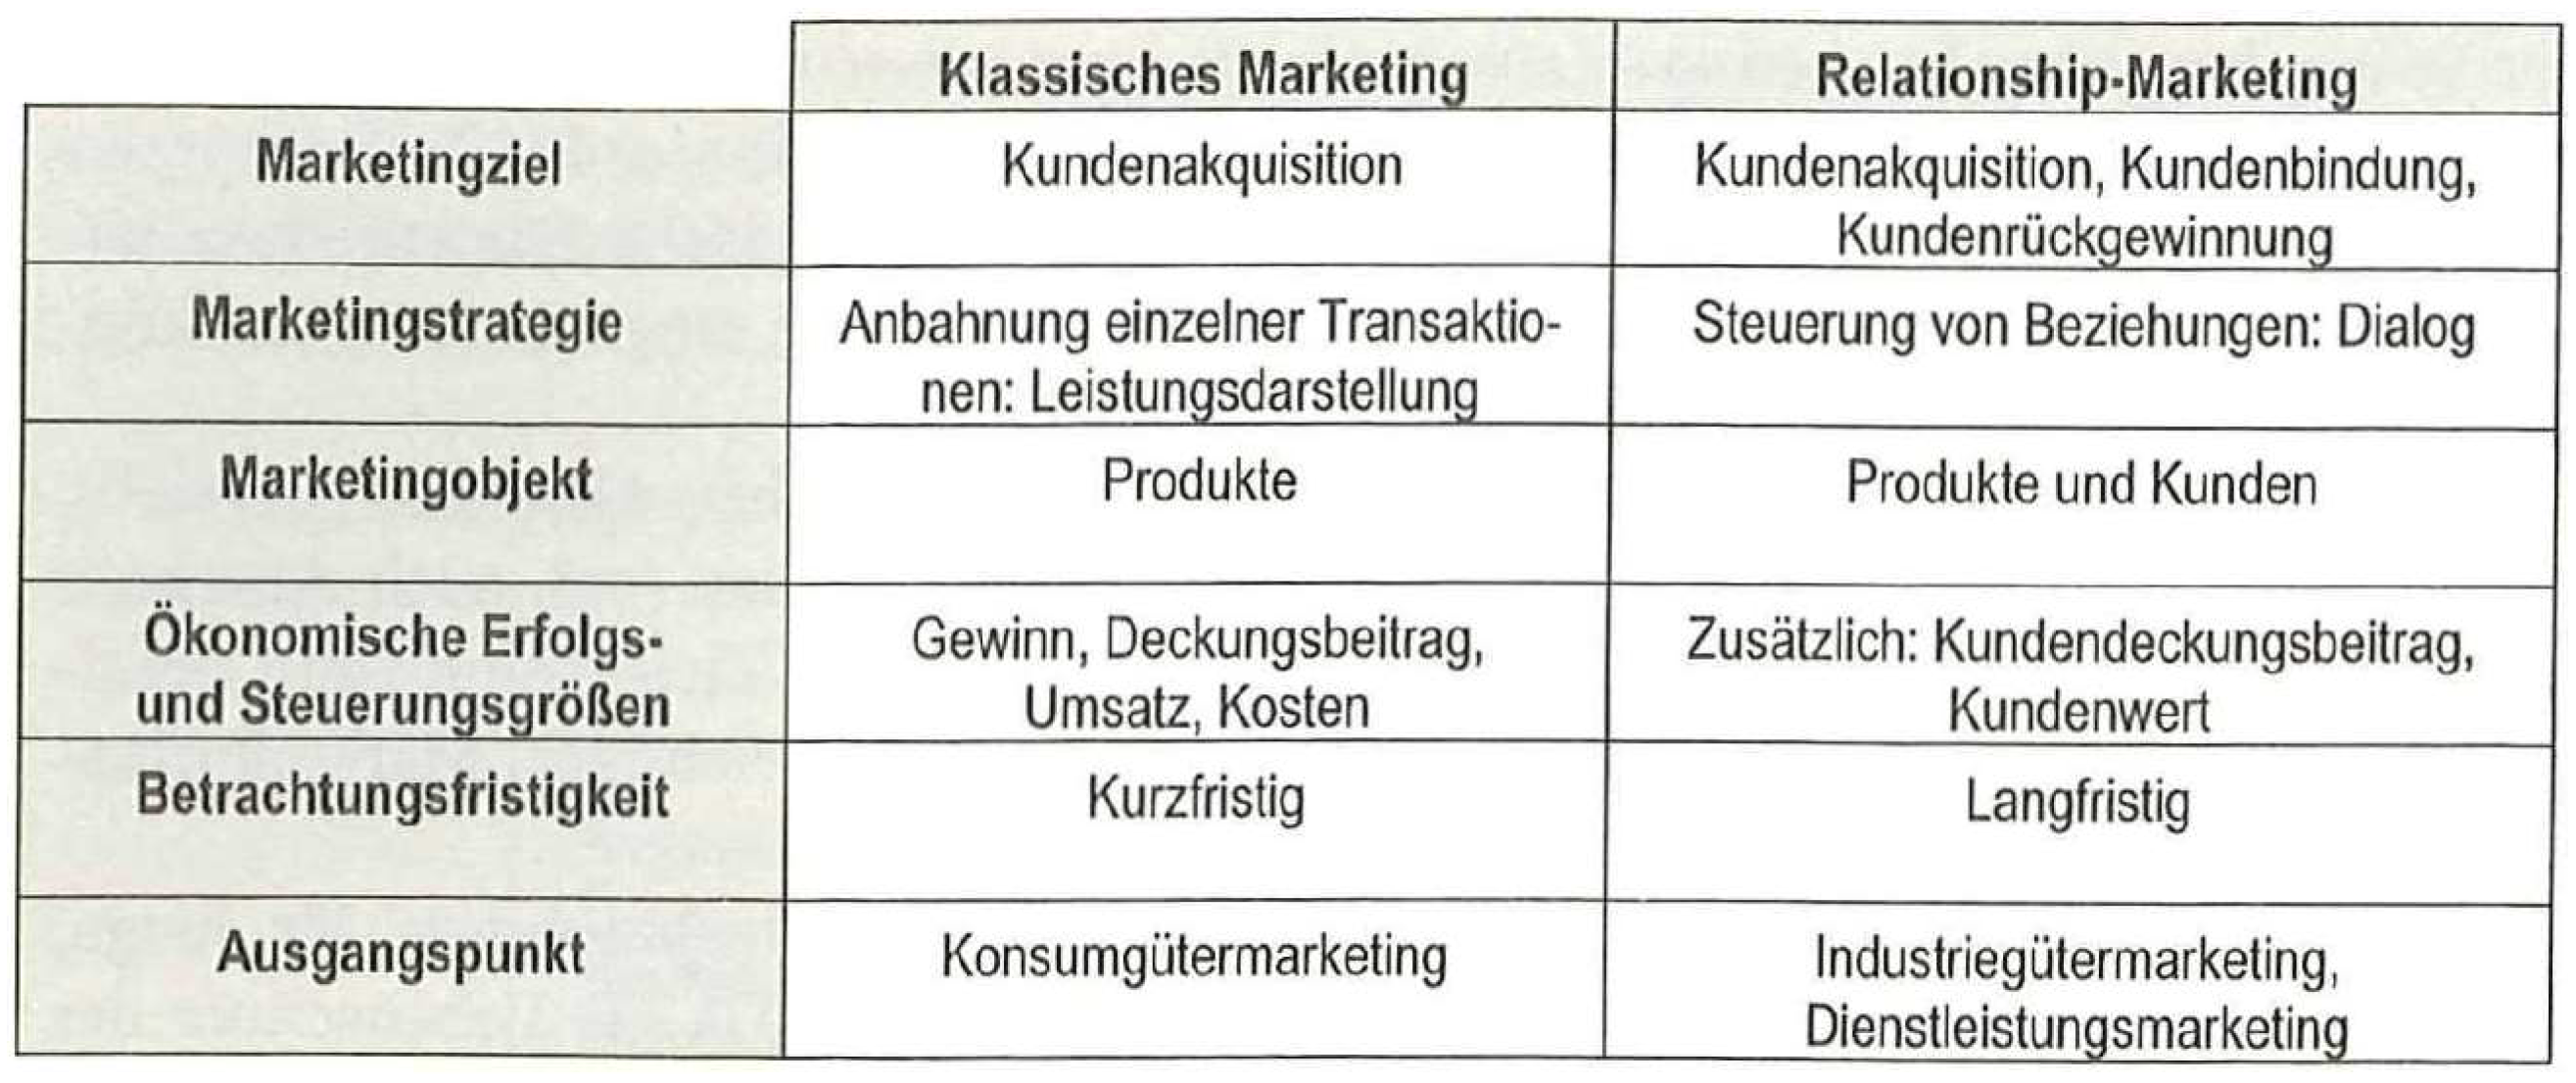
\includegraphics[width=1\linewidth]{images/beziehungsmanagement}
	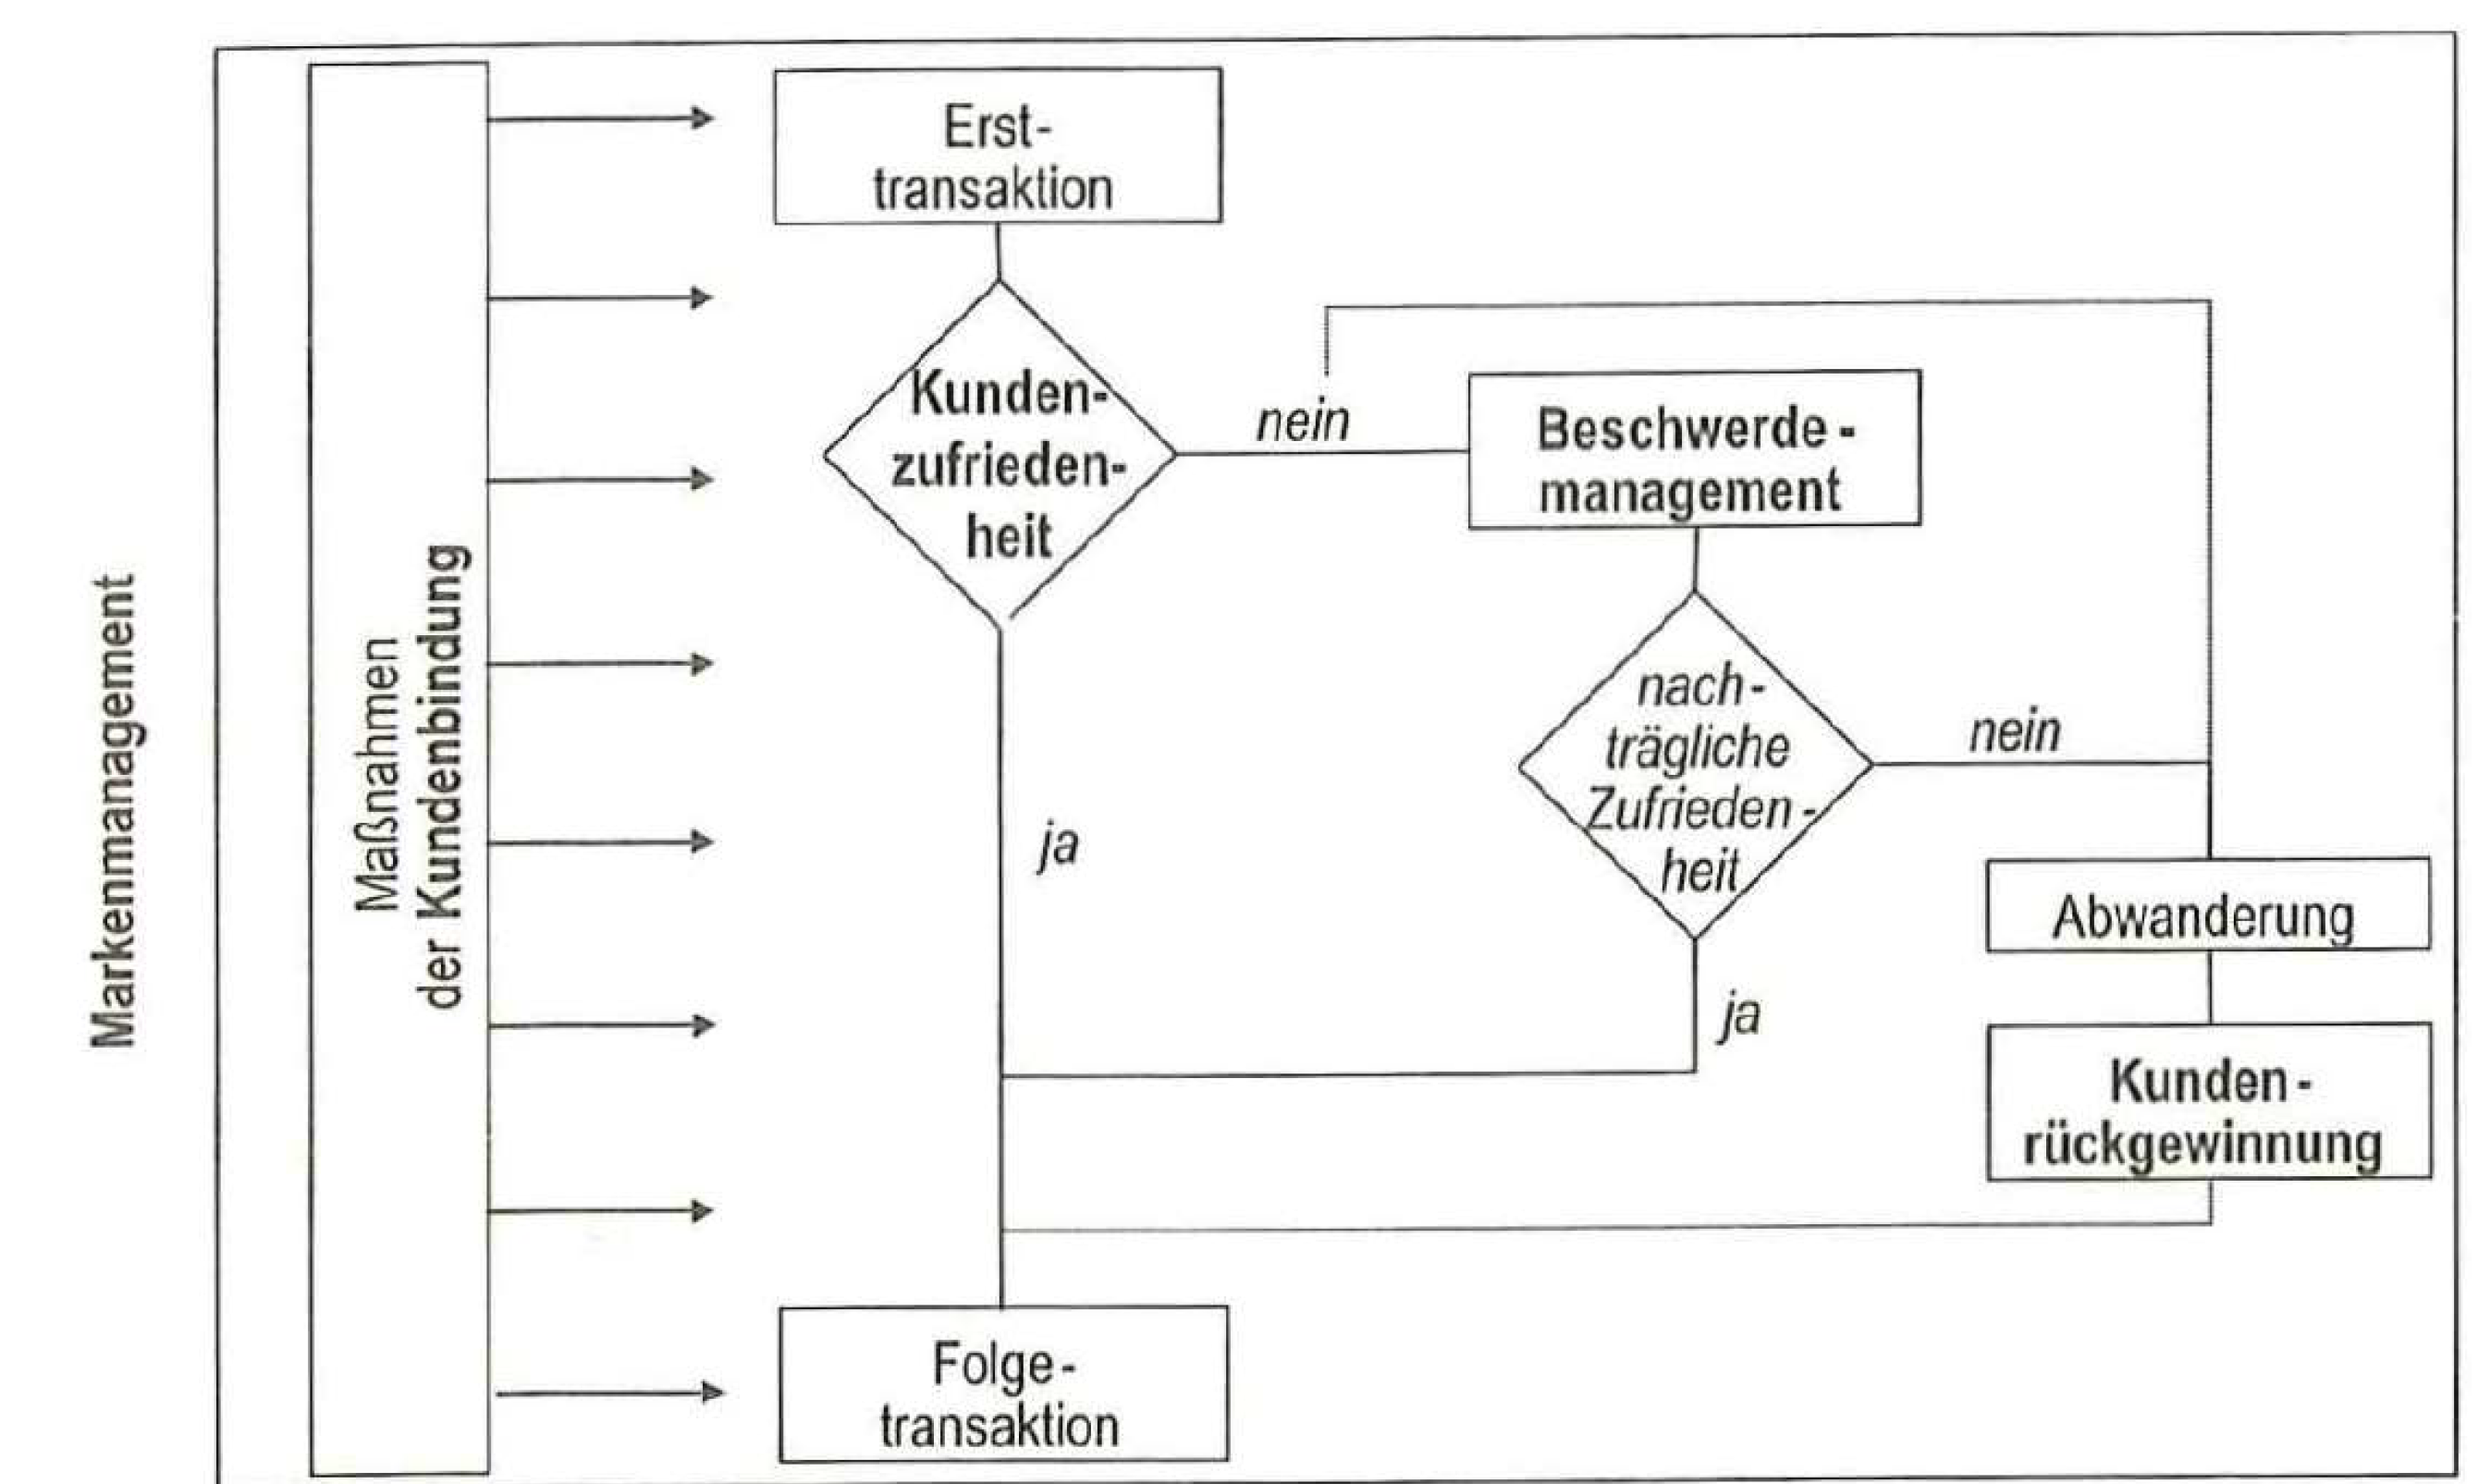
\includegraphics[width=1\linewidth]{images/beziehungsmanagement_2}
\end{multicols}

\paragraph{Markenmanagement}
\begin{itemize}
	\item Marken
	\begin{itemize}
		\item Äusserlich erkennbare Merkmale (z.B. Name, Symbol, Design) die eine Identifizierung eines Produktes / einer Leistung erlauben bzw. dessen Differenzierung vom Wettbewerb
		\item Vorstellungen und Erwartungen (und damit verbundene Wertschätzung und Emotionen), die aufgrund vorheriger Interaktionen und Kommunikation mit der Marke assoziiert werden
	\end{itemize}
	\item Wirkungsweise
	\begin{itemize}
		\item Für Anbieter: «Kommunikationsplattform», die Beziehungsaufbau ermöglicht
		\item Für Nachfrager: Informations-, Vertrauens- und Emotionalisierungsfunktion
		\item Preisprämien und Mengenvorteile (bei Preisgleichheit)
	\end{itemize}
\end{itemize}

\subsection{Marketing-Instrumente}
\subsubsection{Marketing-Mix = 4P}
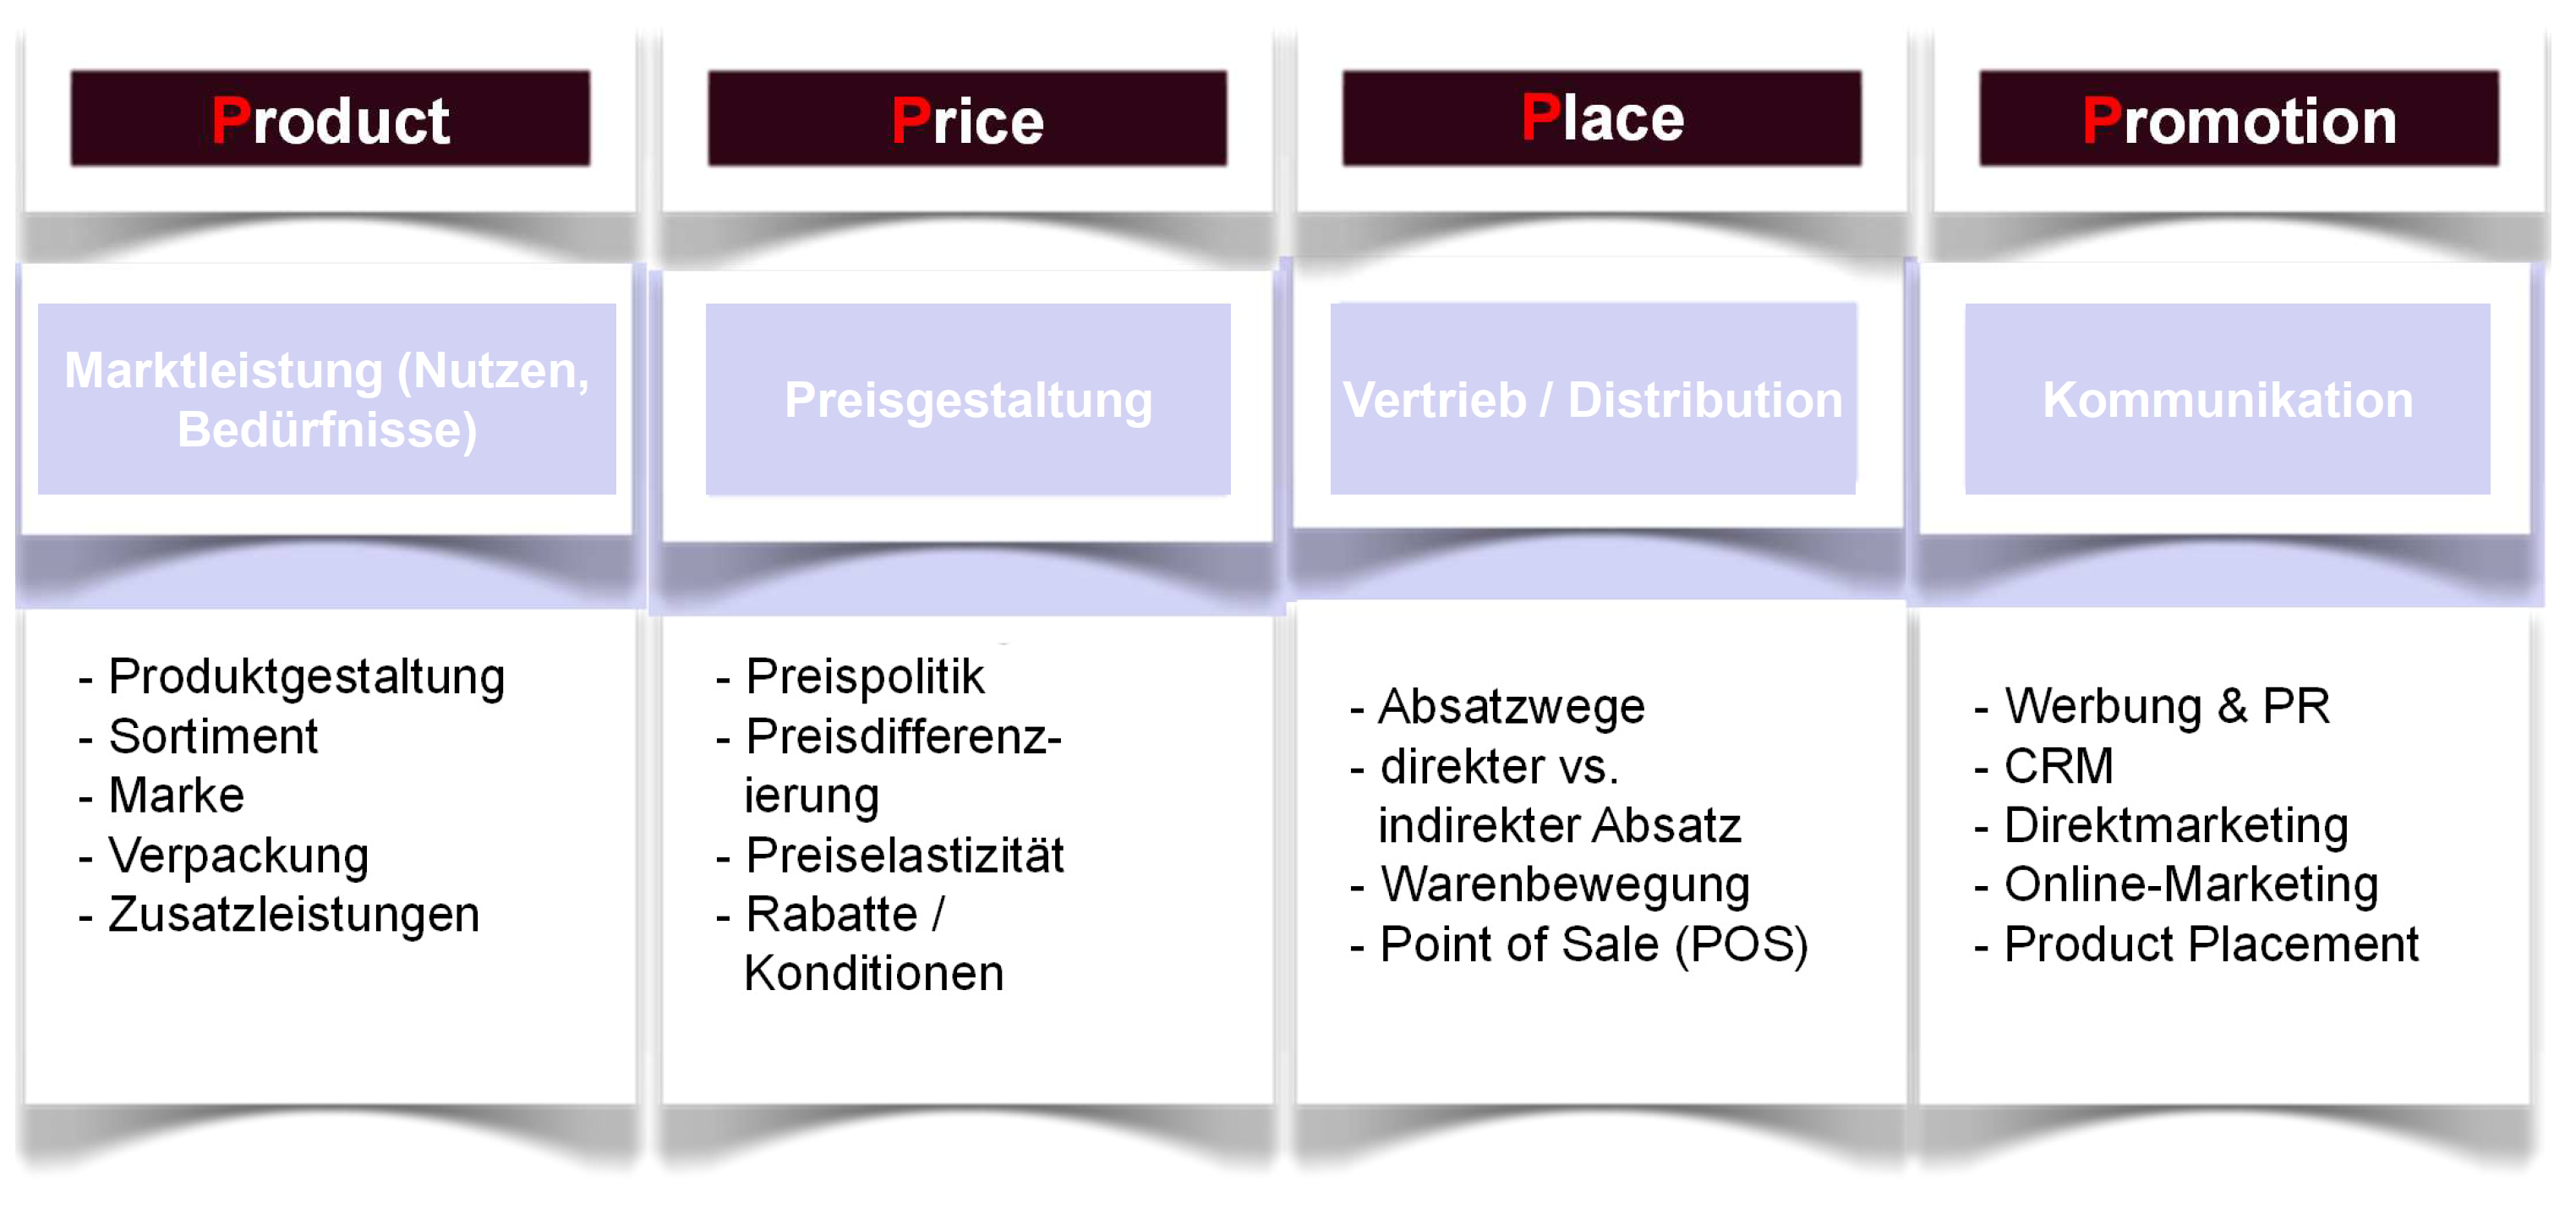
\includegraphics[width=1\linewidth]{images/4p}

\subsubsection{Produktpolitik}
\begin{itemize}
	\item Konzept
	\begin{itemize}
		\item Alle Massnahmen, die auf die Gestaltung des Produktes / der Leistung ausgerichtet sind
		\item Sachliche Entscheidungen (Gestaltung von Bestandteilen)
		\item Zeitlicher Verlauf (Produktlebenszyklen)
	\end{itemize}
	\item Komponenten
	\begin{enumerate}
		\item Produktkern (Erfüllung eines spezifischen Bedürfnisses)
		\item Packung / Verpackung (Schutz, Transport, Lagerung, Promotion,	Umweltverträglichkeit) - Norm
		\item Markierung (Name, Zeichen, Design), Hauptfirma erkennbar
		\item Dienstleistung (Aufwertung, Nichtvergleichbarkeit, zusätzliche Umsätze)
	\end{enumerate}
\end{itemize}

\paragraph{Dienstleistungsklassifizierung}
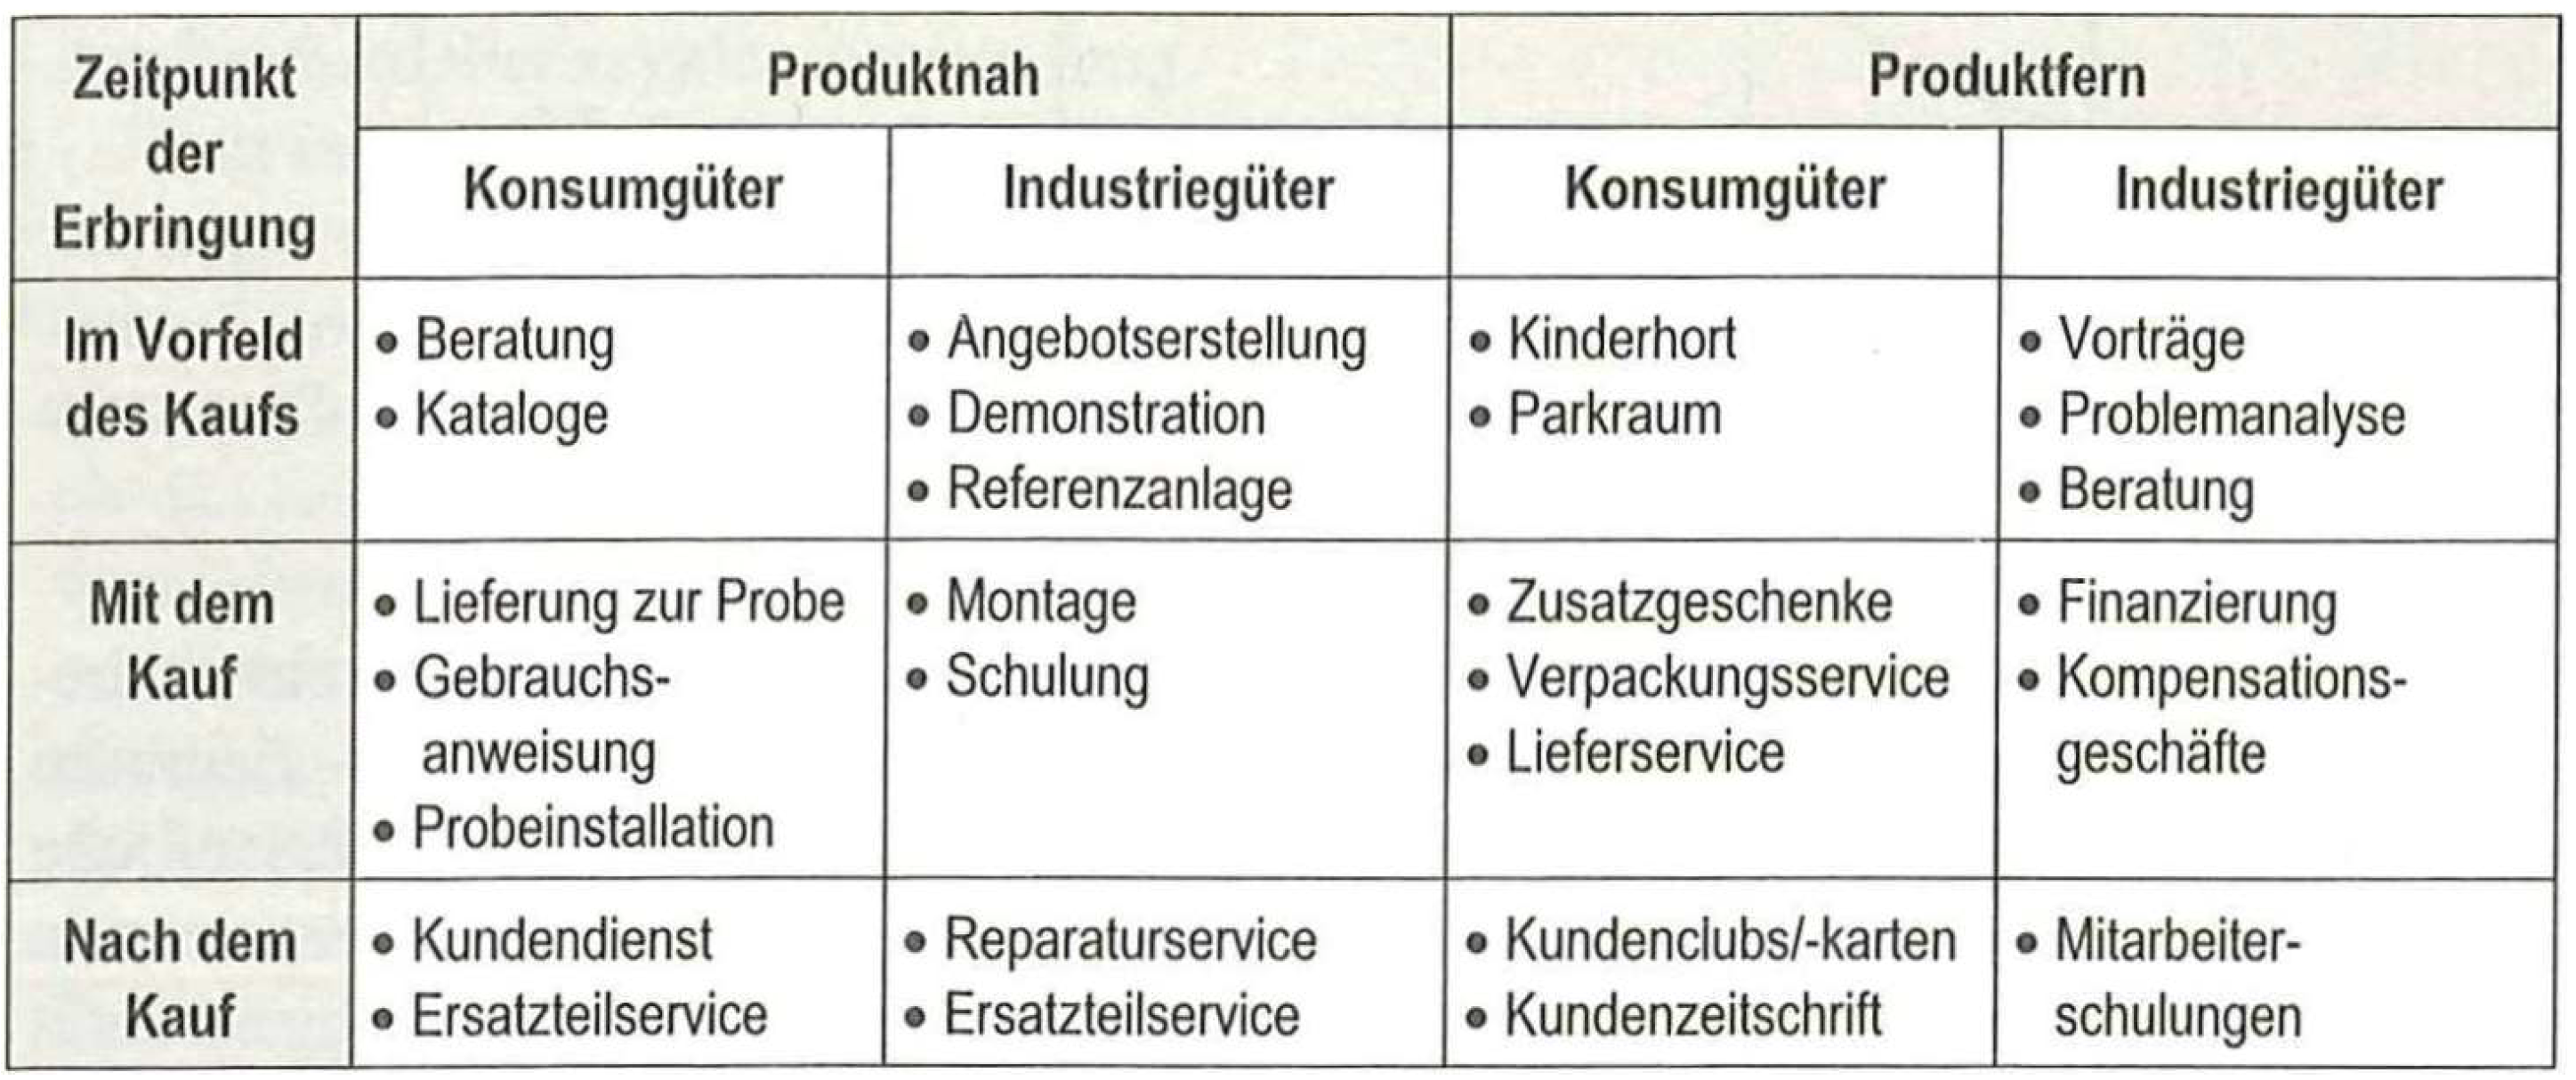
\includegraphics[width=0.8\linewidth]{images/produktpolitik}

\paragraph{Produktlebenszyklen}
\begin{itemize}
	\item Produktinnovationen (Einführungsphase)
	\begin{itemize}
		\item Ideengewinnung (interne und externe Quellen)
		\item Ideenprüfung (Wirtschaftlichkeitsanalysen)
		\item Ideenrealisierung (technische / marktbezogene Tests)
		\item Markteinführung
	\end{itemize}
	\item Produktvariation (Wachstumsphase)
	\begin{itemize}
		\item Leichte Modifikationen am Produkt (Produktvarianten)
		\item Ausweitung auf bisher nicht erreichte Kundensegmente
	\end{itemize}
	\item Produktdifferenzierung (Reifephase)
	\begin{itemize}
		\item Geänderte Markterfordernisse führen zu zunehmender Stagnation
		\item Umfassende Modifikationen am Produkt (Produktvariationen)
	\end{itemize}
	\item Produktelimination (Degenerationsphase)
	\begin{itemize}
		\item Umsatzrückgang ist nicht mehr aufzuhalten
		\item Marktliche und qualitative Faktoren (Image, Konkurrenzreaktion)
	\end{itemize}
\end{itemize}
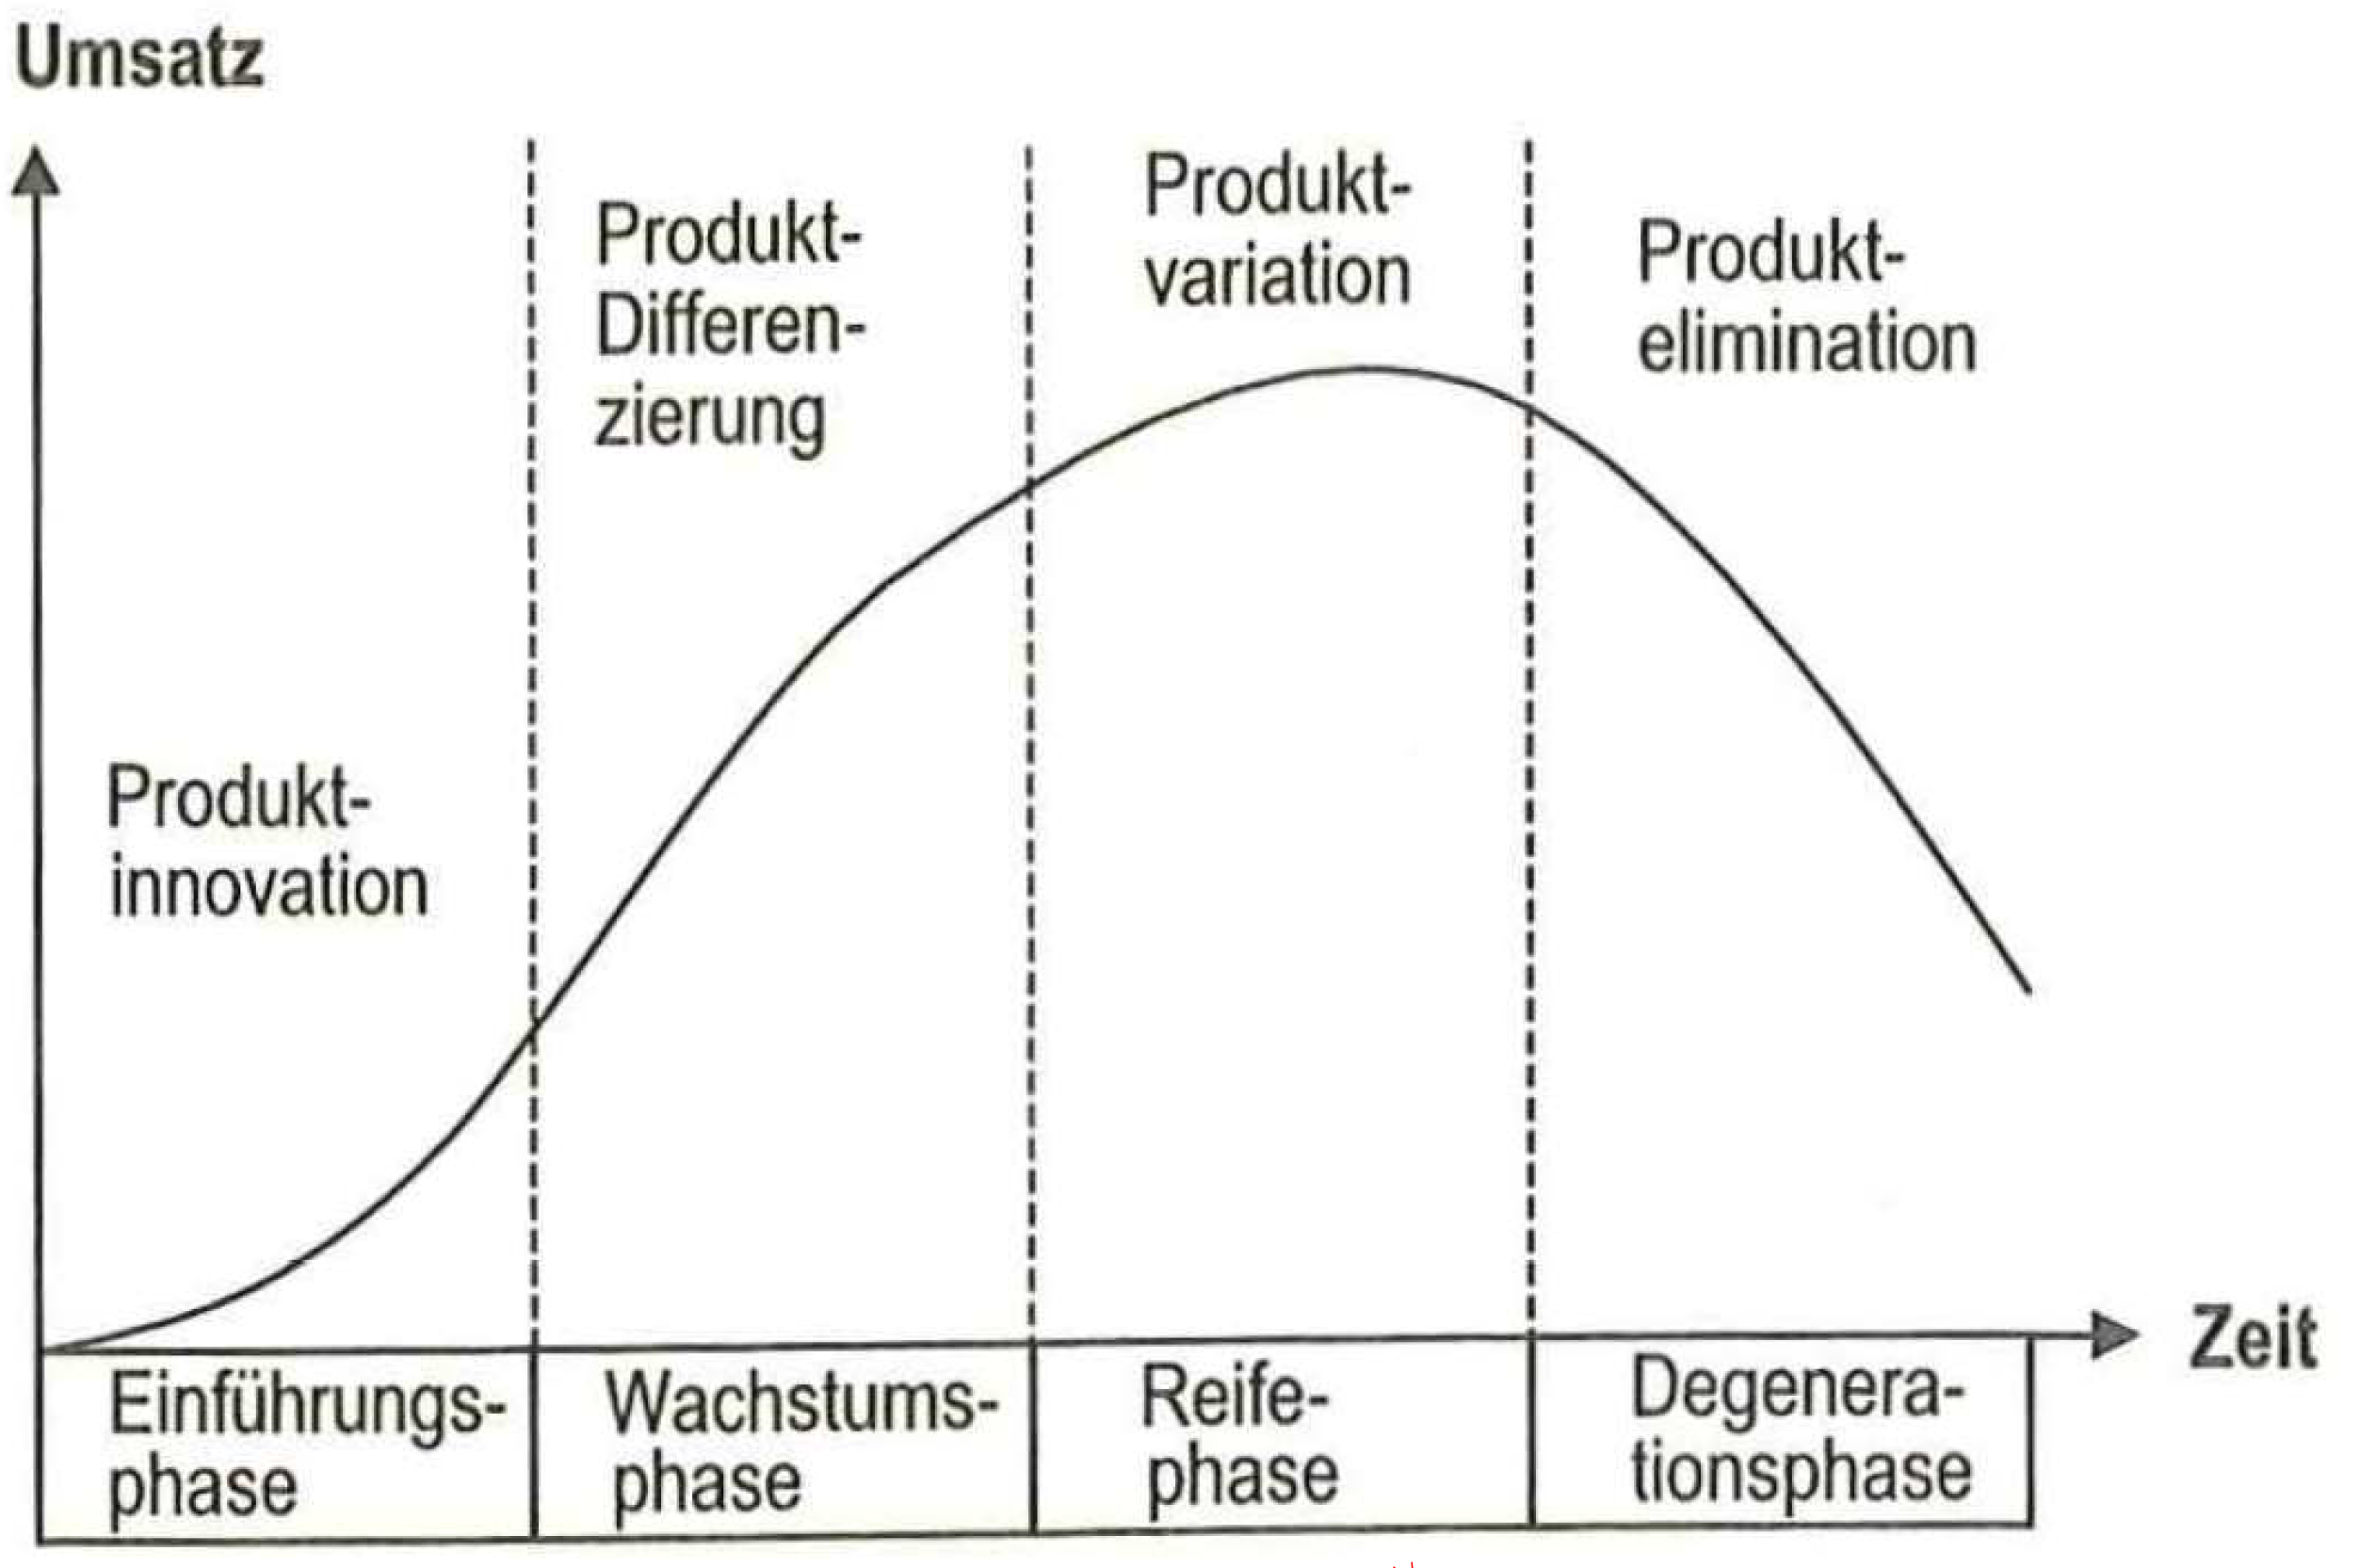
\includegraphics[width=0.5\linewidth]{images/produktlebenszyklen}

